\chapter{Costruzione dell'Optimum Filter e Caratterizzazione del Rumore}
\label{ch:OF}

Negli esperimenti di ricerca diretta di materia oscura come CRESST, la rivelazione di eventi rari e a bassissimo rilascio energetico impone di massimizzare il rapporto segnale-rumore (\textit{Signal-to-Noise Ratio}, SNR). Ottimizzare questo parametro consente di ridurre la soglia energetica del rivelatore ($E_{\text{th}}$), garantendo al tempo stesso un'elevata efficienza di selezione dei segnali fisici e un forte rigetto dei trigger spuri dovuti a fluttuazioni termiche ed elettroniche.

Questo capitolo descrive il percorso adottato per il trattamento dei dati: dalla struttura dei campioni registrati alla formulazione teorica dell'\textit{Optimum Filter} (OF), fino alla determinazione dei suoi due elementi costitutivi — il \textit{Noise Power Spectrum} (NPS) e i template di forma d'onda. Infine (forse), viene presentata l'applicazione del filtro e il criterio di stima del tasso di rumore triggerato in funzione della soglia.

% ==============================================================================
\section{Struttura dei Dati e Parametrizzazione delle Tracce}
\label{sec:struttura_dati}
% ==============================================================================

Nell'esperimento CRESST i segnali vengono acquisiti in modalità continua a una frequenza di campionamento di $25\,\text{kHz}$, che corrisponde a un intervallo temporale tra due campioni consecutivi pari a $\Delta t = 40\,\mu\text{s}$. La registrazione continua consente di applicare algoritmi di filtraggio digitale direttamente sul flusso dati grezzo, per poi applicare in un secondo momento il trigger, riducendo l'impatto del rumore e migliorando la sensibilità sperimentale.

Per monitorare la stabilità della risposta termica del rivelatore e verificarne costantemente il punto di lavoro lungo la transizione superconduttrice del TES (\textit{Transition Edge Sensor}), vengono iniettati periodicamente impulsi di calore artificiali per mezzo di un riscaldatore ohmico (\textit{heater}) integrato sull'assorbitore:
\begin{itemize}
    \item \textbf{TestPulses:} impulsi di calore ad ampiezza variabile programmata (tra $0.1\,\text{V}$ a $10\,\text{V}$ al generatore), impiegati per campionare linearità, guadagno e risoluzione energetica dell'apparato (Figura~\ref{fig:PulsesComparison}b);
    \item \textbf{ControlPulses:} impulsi ad ampiezza fissa ed elevata ($20\,\text{V}$), progettati per portare il film di tungsteno oltre la transizione e saturare la risposta (Figura~\ref{fig:PulsesComparison}a). L'altezza del gradino di saturazione funge da riferimento stabile per correggere eventuali derive termiche del criostato. (Il controlpulse sembra avere stessa ampiezza dell'ultimo Testpulse nonostante ampiezza input registrata sia doppia!!!!)
\end{itemize}

\begin{figure}[htbp]
    \centering
    \begin{minipage}[t]{0.48\textwidth}
        \centering
        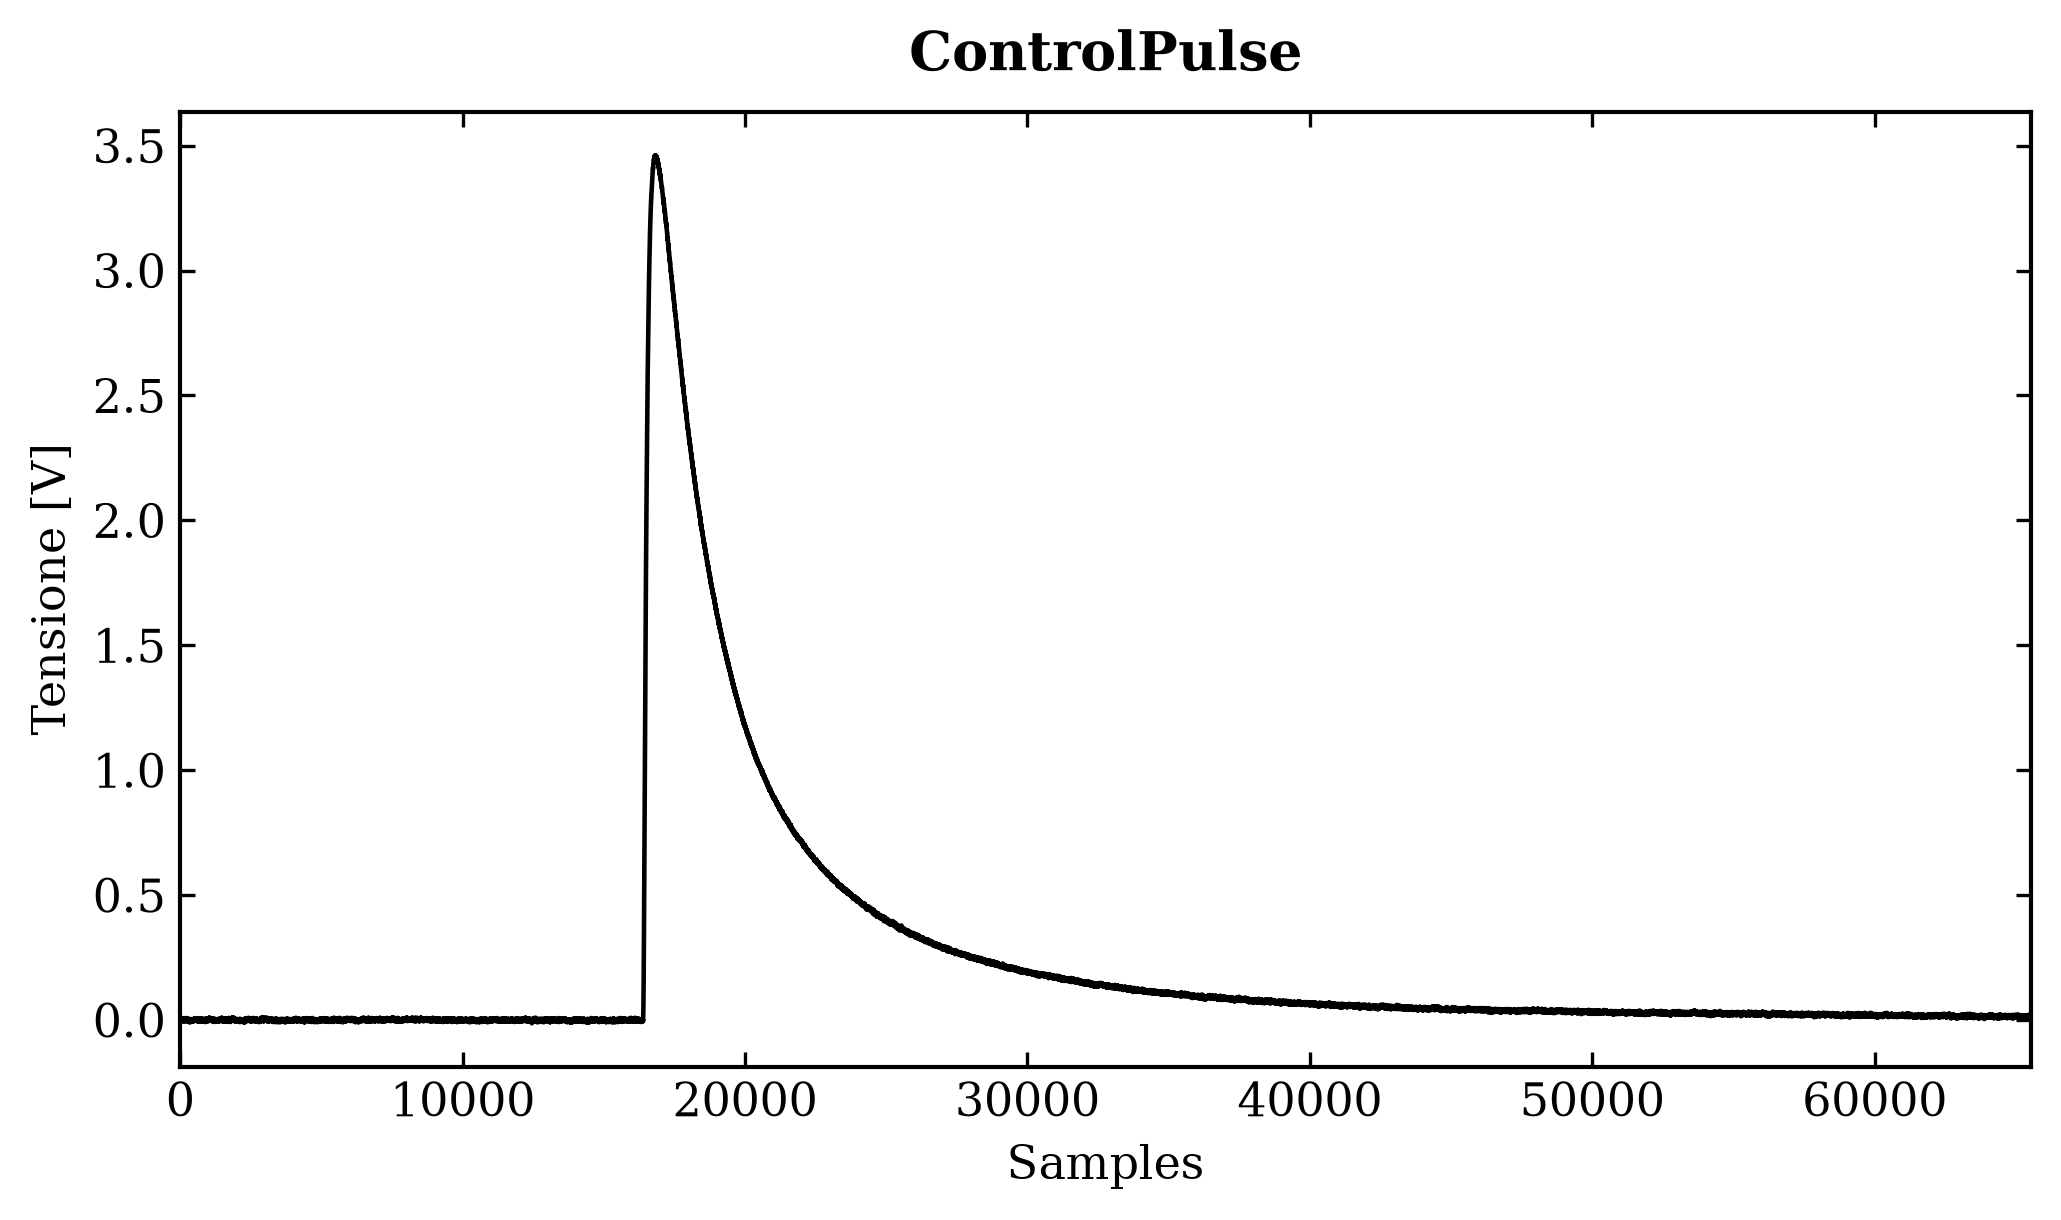
\includegraphics[width=\linewidth]{figures/ControlPulse.png}
        \caption*{(a) Impulso a 20\,V (ControlPulse).}
        \label{fig:ControlPulse}
    \end{minipage}
    \hfill
    \begin{minipage}[t]{0.48\textwidth}
        \centering
        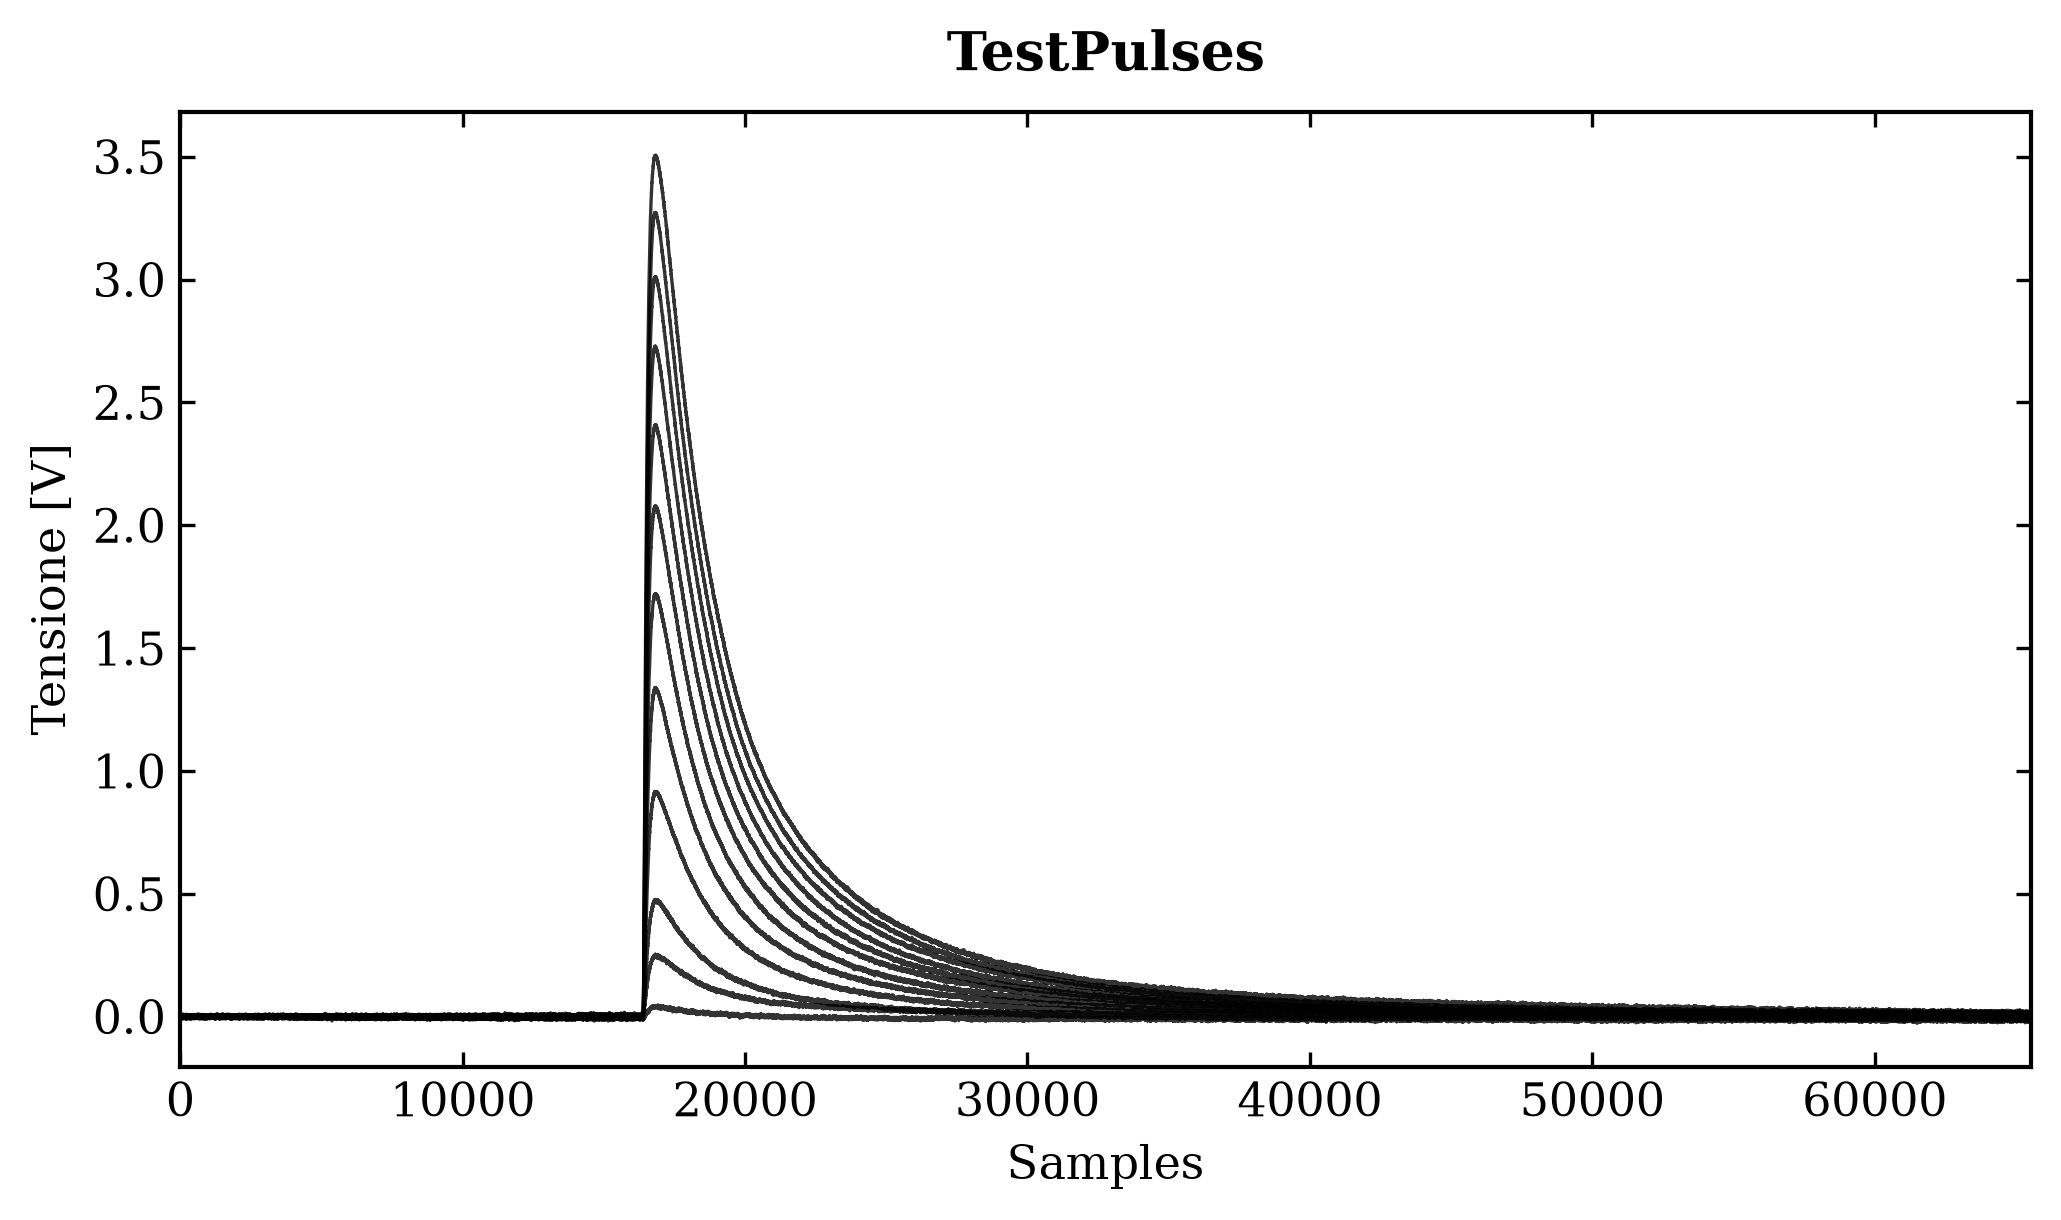
\includegraphics[width=\linewidth]{figures/testpulse.png}
        \caption*{(b) Impulsi tra 0.1\,V e 10\,V (TestPulses).}
        \label{fig:TestPulse}
    \end{minipage}
    \vspace{0.8em}
    \caption{Risposta del sensore agli impulsi iniettati tramite heater: (a) singolo \textit{ControlPulse} saturo a $20\,\text{V}$ e (b) serie di dodici \textit{TestPulses} ad ampiezza variabile campionati lungo l'intervallo di 65536 campioni.}
    \label{fig:PulsesComparison}
\end{figure}

Ogni evento isolato in fase di analisi corrisponde a una finestra temporale di $65536$ campioni (durata complessiva di circa $2.62\,\text{s}$). L'impulso viene convenzionalmente posizionato a un quarto della traccia, attorno al campione $16384$ ($\approx 655.4\,\text{ms}$). Questa asimmetria garantisce un intervallo pre-trigger sufficientemente lungo per stimare il livello e la varianza della linea di base (\textit{baseline}), lasciando al contempo il tempo necessario per registrare il completo rilassamento termico del sistema verso il bagno freddo.

Dalle tracce campionate vengono estratti diversi parametri operativi, riassunti nel seguente elenco e illustrati in Figura~\ref{fig:Parametri_particella}:
\begin{itemize}
    \item \textbf{Baseline Offset:} valore medio della tensione nella finestra pre-trigger, sottratto alla traccia per eliminare la componente continua (DC);
    \item \textbf{Baseline Slope:} pendenza lineare della baseline pre-trigger (unità di misura??);
    \item \textbf{Baseline RMS:} deviazione standard della tensione nella regione prima dell'evento;
    \item \textbf{Baseline Difference:} differenza tra la media della tensione prima dell'impulso e quella a fine finestra;
    \item \textbf{Rise Time (RT):} tempo impiegato dal fronte di salita per passare dal $x\%$ al $x\%$ dell'altezza massima;
    \item \textbf{Decay Time (DT):} tempo impiegato dalla coda del segnale per scendere dal $x\%$ al $x\%$ del picco;
    \item \textbf{Peak Position:} coordinata temporale del massimo assoluto identificato lungo la finestra.
\end{itemize}

\begin{figure}[htbp]
    \centering
    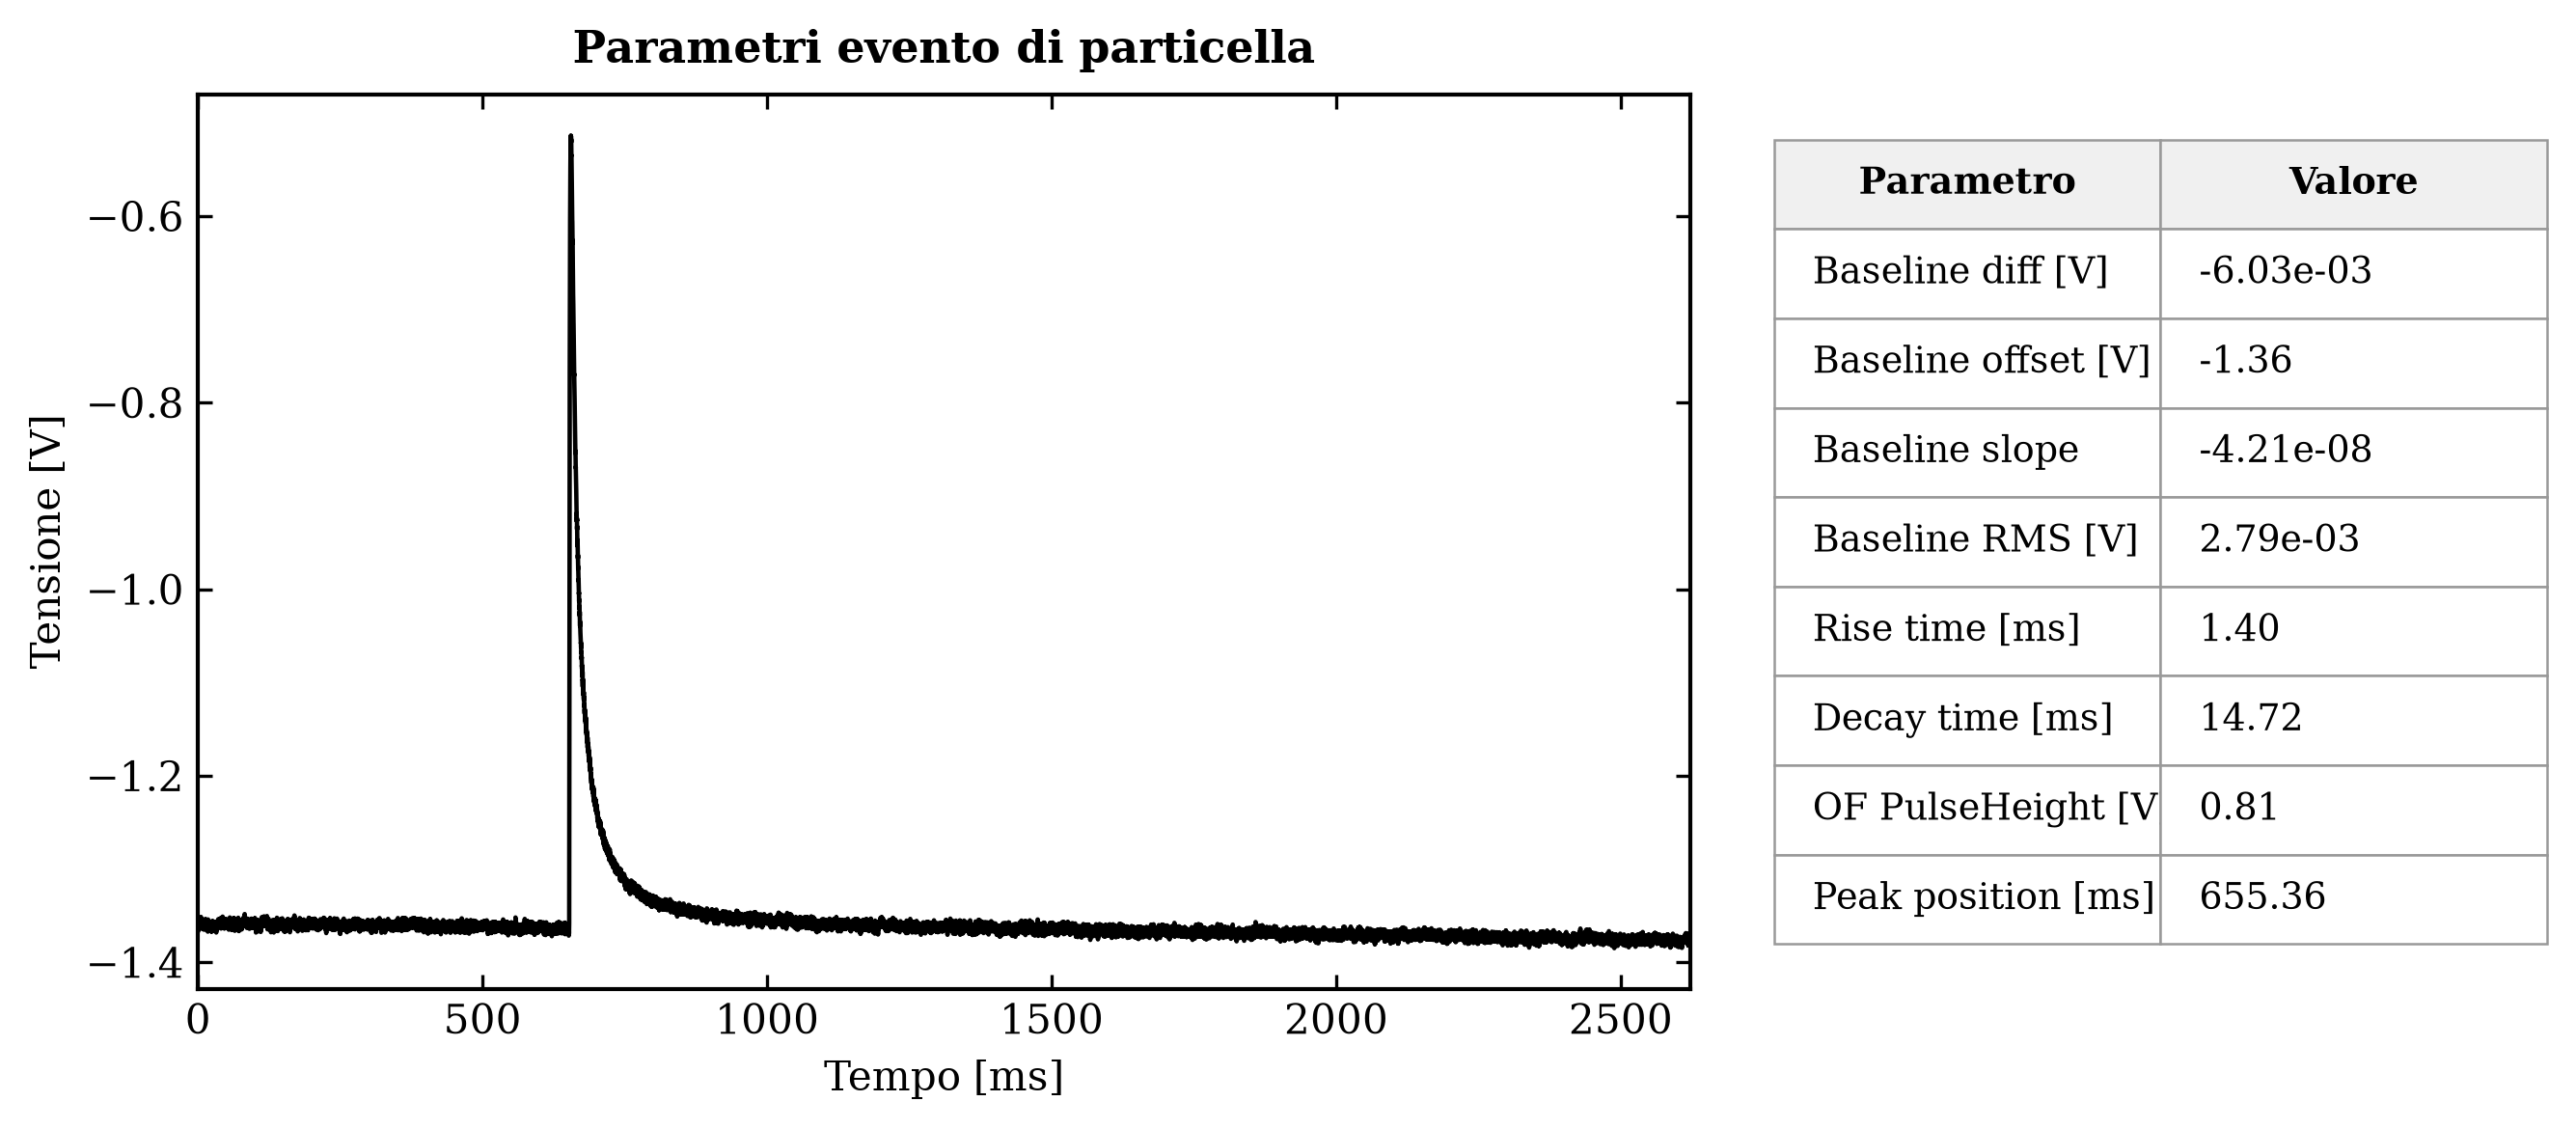
\includegraphics[width=0.95\textwidth]{figures/Parametri_particella.png}
    \caption{Esempio di traccia di particella registrata nel cristallo (a sinistra) e relativa tabella dei parametri di forma calcolati (a destra). (Sistemare unità di misura!!!!)}
    \label{fig:Parametri_particella}
\end{figure}

% ==============================================================================
\section{Formalismo Teorico dell'Optimum Filter}
\label{sec:teoria_OF}
% ==============================================================================

Il metodo più immediato per ricavare l'energia depositata da un'interazione consisterebbe nel campionare il valore massimo della traccia dopo aver rimosso l'offset della baseline. Tuttavia, in presenza di segnali di piccola ampiezza confrontabili con l'RMS del fondo, il massimo misurato tende a coincidere con la somma tra l'impulso reale e la più alta fluttuazione casuale positiva presente in quel punto. Questo effetto introduce una sovrastima sistematica dell'ampiezza.

Per ovviare al problema si adotta l'\textit{Optimum Filter} (OF), sviluppato originariamente da Gatti e Manfredi ~\cite{gatti_manfredi}. L'algoritmo sfrutta il fatto che, in regime di risposta lineare del sensore, gli impulsi condividono una forma d'onda comune e differiscono unicamente per un fattore di scala proporzionale all'energia. Una traccia misurata $v(t)$, depurata dall'offset continuo, viene quindi modellata come:
\begin{equation}
    v(t) = A \cdot s(t - t_0) + n(t)
    \label{eq:segnale_modello}
\end{equation}
dove $s(t)$ è la forma d'onda attesa normalizzata a massimo unitario (\textit{template}), $A$ è l'ampiezza incognita da stimare, $t_0$ è l'istante di arrivo del segnale ed $n(t)$ è il rumore stocastico additivo sovrapposto.

L'Optimum Filter opera nello spazio delle frequenze tramite una funzione di trasferimento $H(f)$ costruita per massimizzare il rapporto tra l'ampiezza dell'impulso e il rumore di fondo. Tale funzione assume la forma:
\begin{equation}
    H(f) = K \frac{S^*(f)}{N(f)} e^{-i 2\pi f t_0}
    \label{eq:OF_transfer_function}
\end{equation}
dove:
\begin{itemize}
    \item $S^*(f)$ è il complesso coniugato della trasformata di Fourier del template $s(t)$, che pesa maggiormente le bande di frequenza in cui si concentra la potenza del segnale fisico;
    \item $N(f)$ è la densità di potenza del rumore (\textit{Noise Power Spectrum}, NPS), che ha il compito di ridurre le frequenze dominate da disturbi sperimentali;
    \item $e^{-i 2\pi f t_0}$ compensa lo sfasamento temporale dell'evento lungo la traccia;
    \item $K$ è una costante reale di normalizzazione definita come:
    \begin{equation}
        K = \left( \int_{-\infty}^{+\infty} \frac{|S(f)|^2}{N(f)} \, df \right)^{-1}
        \label{eq:costante_normalizzazione}
    \end{equation}
    Poiché i segnali sperimentali vengono acquisiti a tempo discreto su un intervallo finito di $N$ campioni, l'integrale viene valutato numericamente tramite sommatoria sui bin di frequenza discreti $f_k = k \cdot \Delta f$ (con $\Delta f = f_camp / N$). Sfruttando la proprietà per cui il modulo quadro della trasformata di Fourier di un segnale reale è una funzione pari rispetto all'origine ($|S(-f)|^2 = |S(f)|^2$), l'integrazione sulle frequenze negative si ripiega su quelle positive:
    \begin{equation}
        K = \left[ \Delta f \left( \frac{|S(0)|^2}{N(0)} + 2 \sum_{k=1}^{N/2 - 1} \frac{|S(f_k)|^2}{N(f_k)} + \frac{|S(f_{\text{Nyq}})|^2}{N(f_{\text{Nyq}})} \right) \right]^{-1}
        \label{eq:costante_normalizzazione_discreta}
    \end{equation}
dove $f_{\text{Nyq}} = f_{N/2} = f_s / 2$ rappresenta la frequenza di Nyquist, che, insieme alla componente continua ($k=0$), è l'unica a comparire con peso unitario in quanto non possiedono una controparte simmetrica nell'intervallo fondamentale.
\end{itemize}

Una volta calcolata $H(f)$, la traccia filtrata nel tempo si ottiene applicando l'antitrasformata di Fourier al prodotto tra lo spettro del segnale grezzo $V(f)$ e il filtro:
\begin{equation}
    v_{\text{filt}}(t) = \mathcal{F}^{-1} \Big[ V(f) \cdot H(f) \Big]
\end{equation}
Il massimo di $v_{\text{filt}}(t)$ fornisce la stima ottimale dell'ampiezza cercata ${A}$ (\ref{eq:segnale_modello}), indicata come \textit{Optimum Filter Pulse Height}, mentre l'istante in cui cade tale picco identifica il parametro \textit{Peak Position}.

% ==============================================================================
\section{Caratterizzazione del Rumore e Stima del Noise Power Spectrum}
\label{sec:costruzione_NPS}
% ==============================================================================

Per calcolare il denominatore della funzione di trasferimento dell'OF è necessario stimare sperimentalmente la densità spettrale $N(f)$ a partire da finestre temporali registrate in assenza di segnale fisico.

Durante il funzionamento continuo, le inevitabili derive termiche a bassissima frequenza dell'apparato criogenico provocano variazioni della linea di base. Se una finestra di rumore presenta una deriva non nulla, i livelli di tensione all'inizio e alla fine risulteranno disallineati. Poiché la Trasformata Discreta di Fourier (DFT) tratta implicitamente il record come una sequenza periodica, il disallineamento tra i due estremi viene interpretato come una discontinuità a gradino. Tale gradino introduce una forte componente spuria a bassa frequenza, che distorce e sovrastima lo spettro del rumore, come illustrato in Figura~\ref{fig:gradino}.

\begin{figure}[htbp]
    \centering
    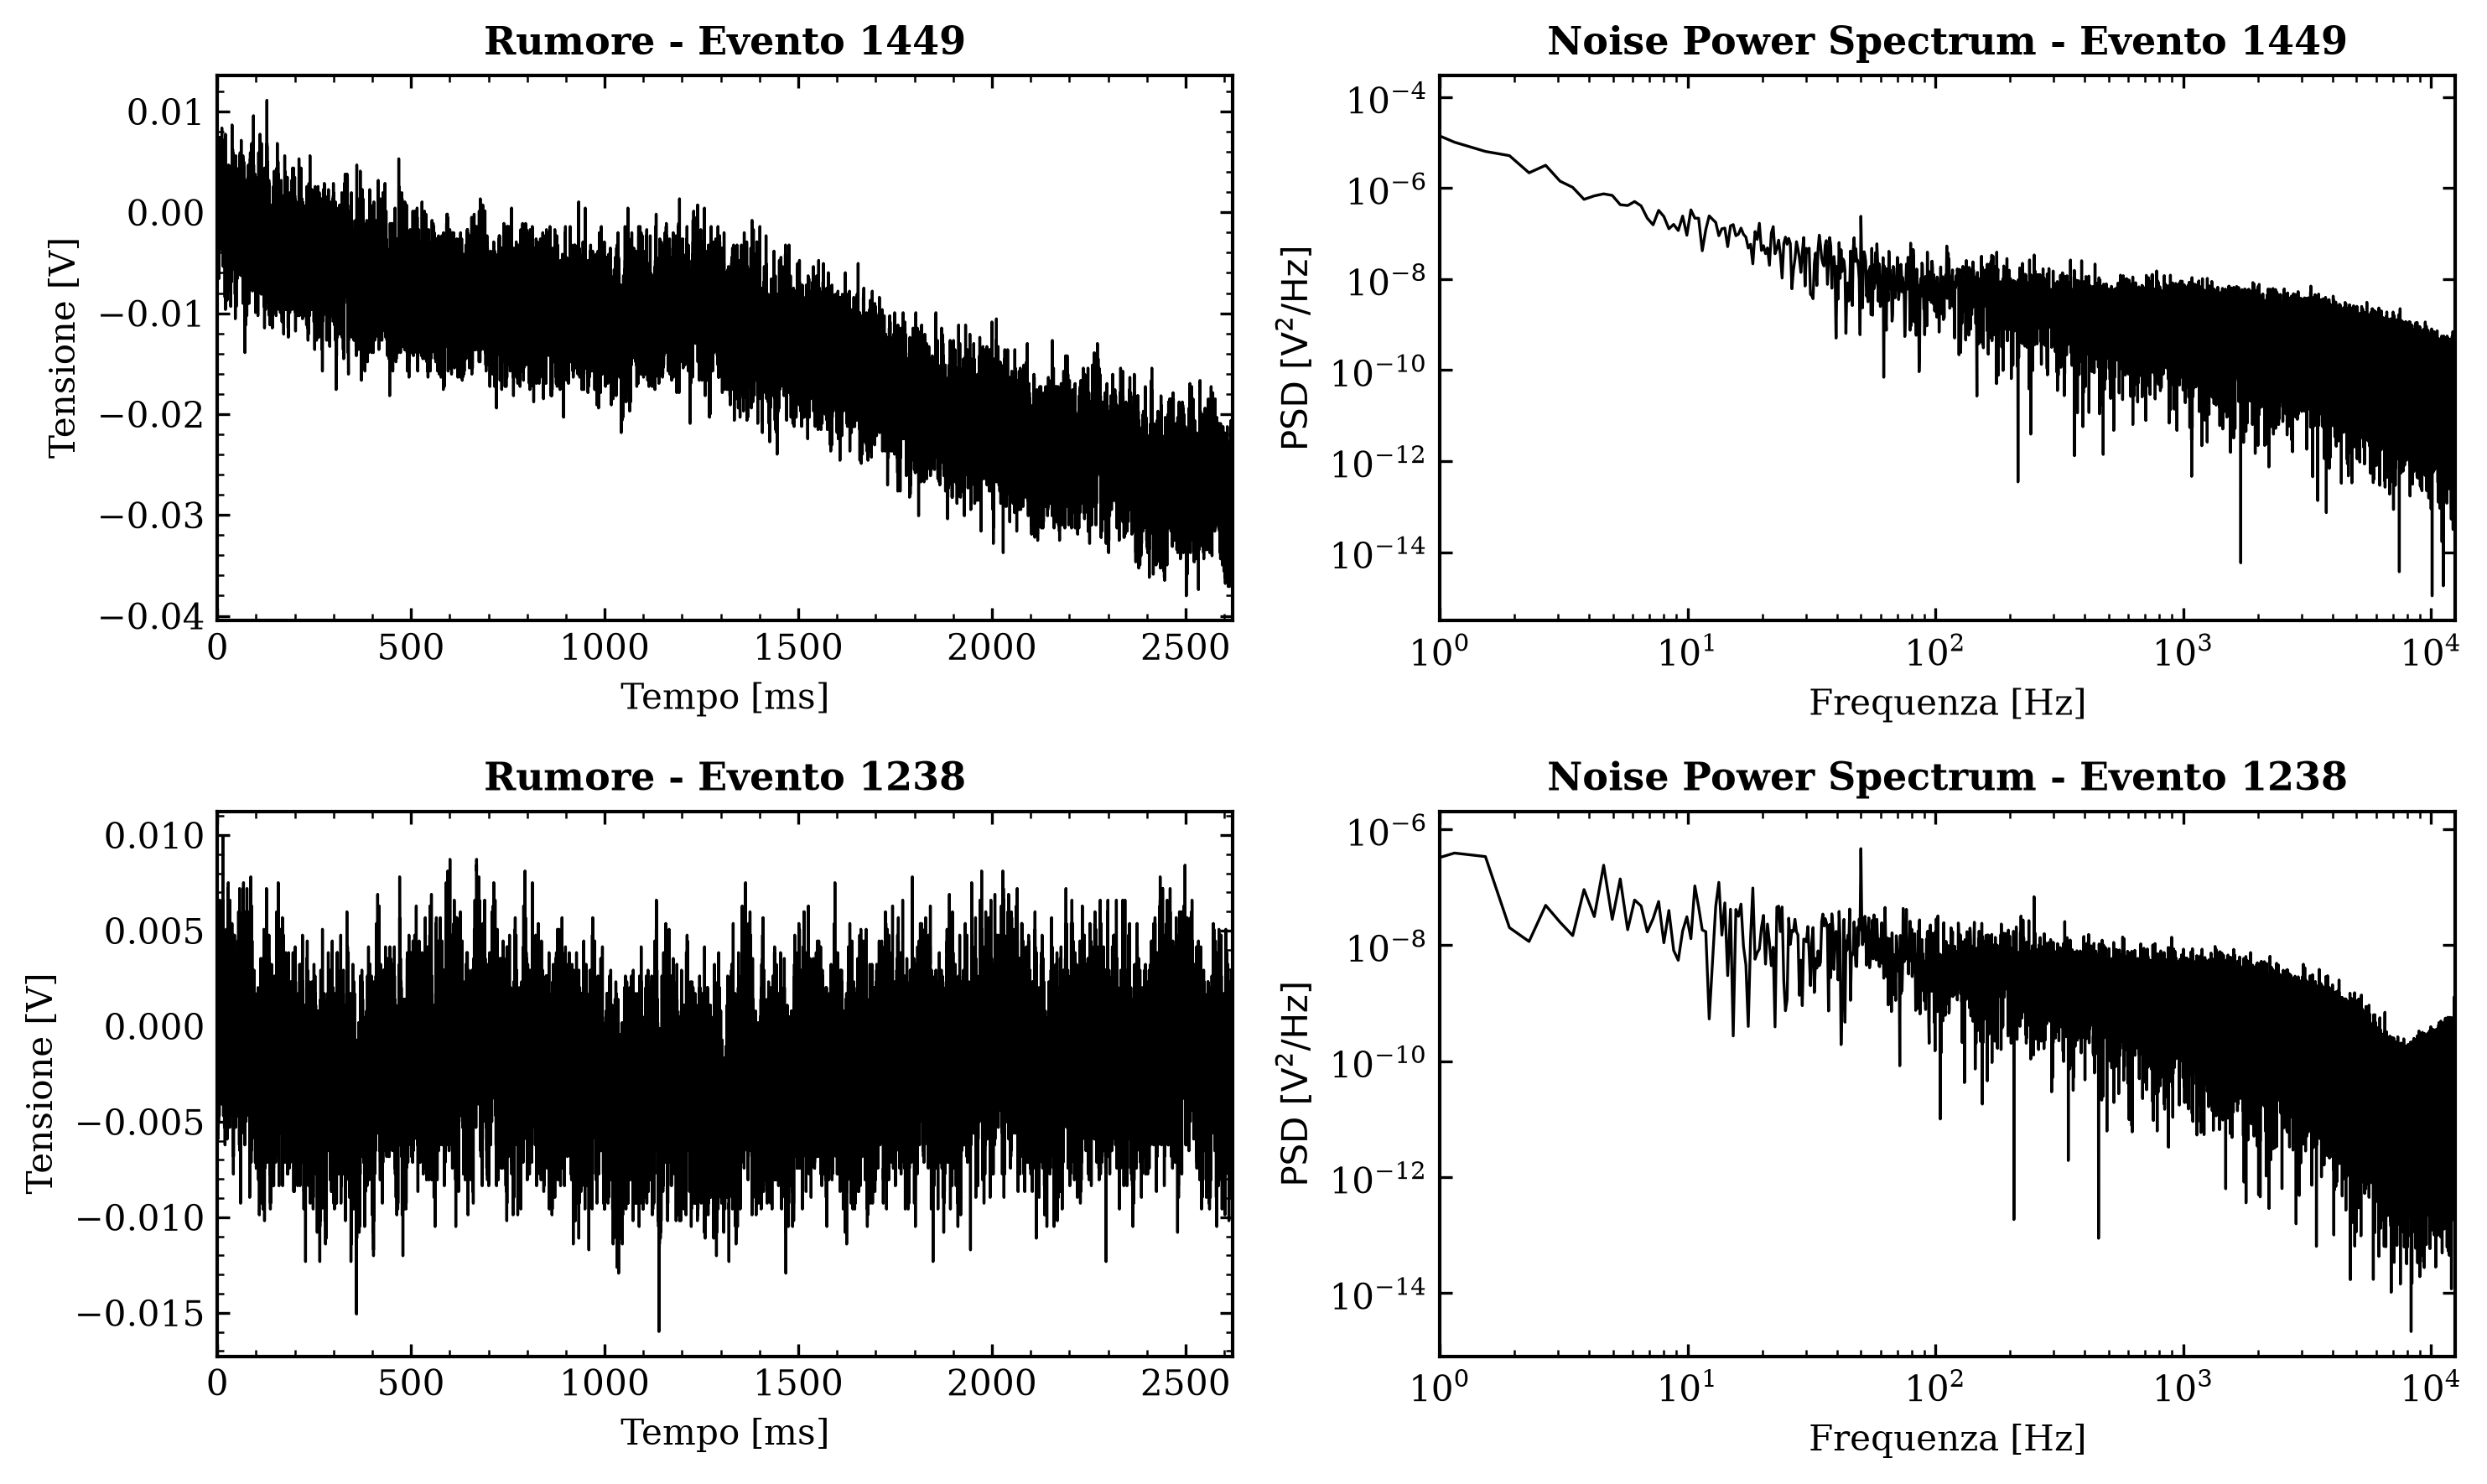
\includegraphics[width=0.9\textwidth]{figures/NPS_baselines.png}
    \caption{Confronto tra due tracce di rumore: l'evento superiore risente di una deriva di baseline che produce un gradino tra i margini, generando nello spettro un'iniezione fittizia di potenza a bassa frequenza; l'evento inferiore, piatto e stazionario, restituisce il profilo indisturbato del rumore.}
    \label{fig:gradino}
\end{figure}

Per selezionare esclusivamente tracce di rumore stazionarie, il campione iniziale viene depurato applicando una serie di criteri di selezione:
\begin{itemize}
    \item \textbf{Pulse Height $< 4\,\text{mV}$:} esclude piccoli impulsi fisici o transienti spuri sfuggiti al trigger;
    \item \textbf{Baseline Difference $< 0.5\,\text{mV}$:} rigetta eventi che contengono code termiche o fluttuazioni a gradino;
    \item \textbf{Fit polinomiale di terzo grado:} la traccia viene modellata con un polinomio cubico. Si conservano solo gli eventi con coefficienti compresi tra il $10^\circ$ e il $90^\circ$ percentile della distribuzione, eliminando andamenti non lineari anomali.
\end{itemize}

Sulle tracce accettate si sottrae il fit cubico per rimuovere ogni pendenza residua (\textit{detrending}). Si calcola quindi la trasformata $V_i(f)$ per ciascuna delle $M$ tracce selezionate e si valuta la Densità Spettrale di Potenza a frequenze positive:
\begin{equation}
    N(f) = \frac{2}{N f_s} \frac{1}{M} \sum_{i=1}^{M} |V_i(f)|^2
\end{equation}
dove $N = 65536$ è il numero di campioni, $f_s = 25\,\text{kHz}$ è la frequenza di campionamento e il fattore 2 preserva la potenza totale piegando le frequenze negative su quelle positive.

\begin{figure}[htbp]
    \centering
    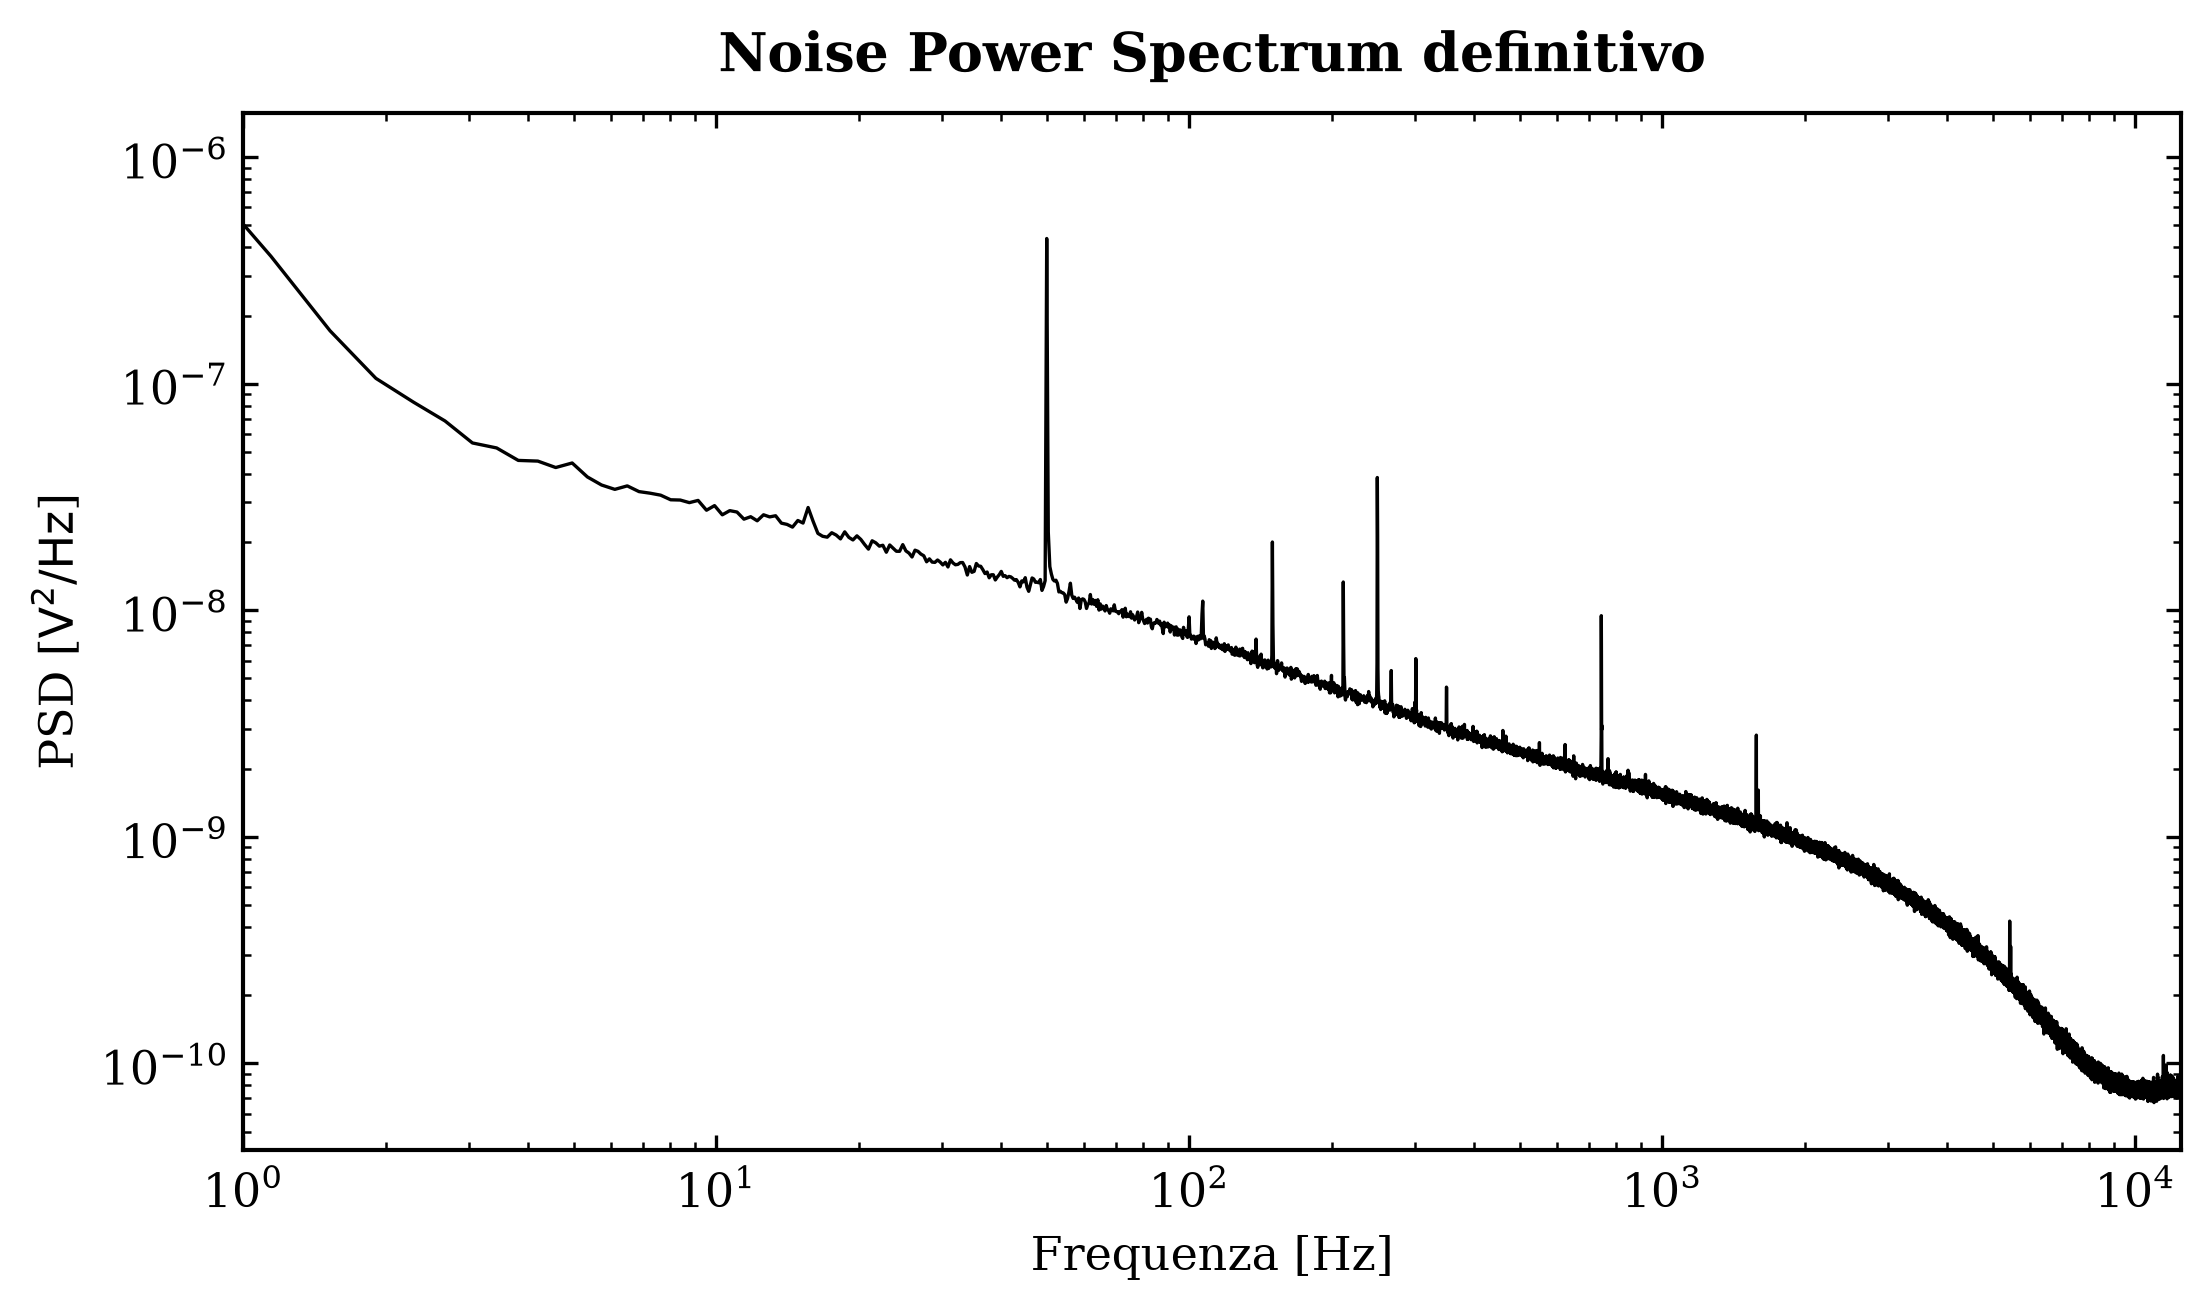
\includegraphics[width=0.9\textwidth]{figures/NPS.png}
    \caption{\textit{Noise Power Spectrum} ottenuto dalla media e normalizzazione di circa 1000 eventi di rumore depurati con fit di terzo grado.}
    \label{fig:NPS}
\end{figure}

Lo spettro finale (Figura~\ref{fig:NPS}) evidenzia chiaramente i contributi del rumore di fondo: oltre a una componente continua a bassa frequenza, emergono il picco fondamentale della rete a $50\,\text{Hz}$ e le relative armoniche dispari ($150\,\text{Hz}$ e $250\,\text{Hz}$), dovute a captazioni elettromagnetiche e ground loop. Inserito a denominatore nella funzione di trasferimento $H(f)$, $N(f)$ smorza selettivamente queste frequenze, eliminando le interferenze periodiche dalla stima dell'ampiezza.

% ==============================================================================
\section{Costruzione dei Template di Segnale}
\label{sec:costruzione_template}
% ==============================================================================

Il numeratore dell'Optimum Filter richiede la conoscenza della forma d'onda di riferimento $s(t)$ (\ref{eq:segnale_modello}). Poiché i canali di eccitazione del rivelatore sono due, particelle ionizzanti che interagiscono nel volume del cristallo e impulsi termici iniettati sull'heater, è necessario definire due template separati.

% ------------------------------------------------------------------------------
\subsection{Template Fononico per Eventi Fisici}
\label{subsec:template_fononico}

Per ricavare il template del segnale particellare, l'obiettivo è mediare un insieme numericamente consistente di tracce pulite, in modo da cancellare il rumore stocastico e isolare la dinamica termica pura. 

A questo scopo sono stati selezionati eventi prodotti da una sorgente esterna di calibrazione di $^{55}\text{Fe}$. Il decadimento per cattura elettronica del $^{55}\text{Fe}$ genera raggi X caratteristici a circa $5.9\,\text{keV}$ ($K_\alpha$) e $6.4\,\text{keV}$ ($K_\beta$). Questa energia è ideale: è sufficientemente elevata da emergere nettamente dal rumore di fondo, ma abbastanza contenuta da non saturare il sensore TES, garantendo una risposta strettamente lineare.

Gli eventi vengono selezionati richiedendo una \textit{pulse height} preliminare compresa tra $0.8\,\text{V}$ e $0.9\,\text{V}$ (intervallo corrispondente al picco del ferro), assenza di derivate negative anomale (generate da disturbi dell'elettronica) e stabilità della linea di base.

\begin{figure}[htbp]
    \centering
    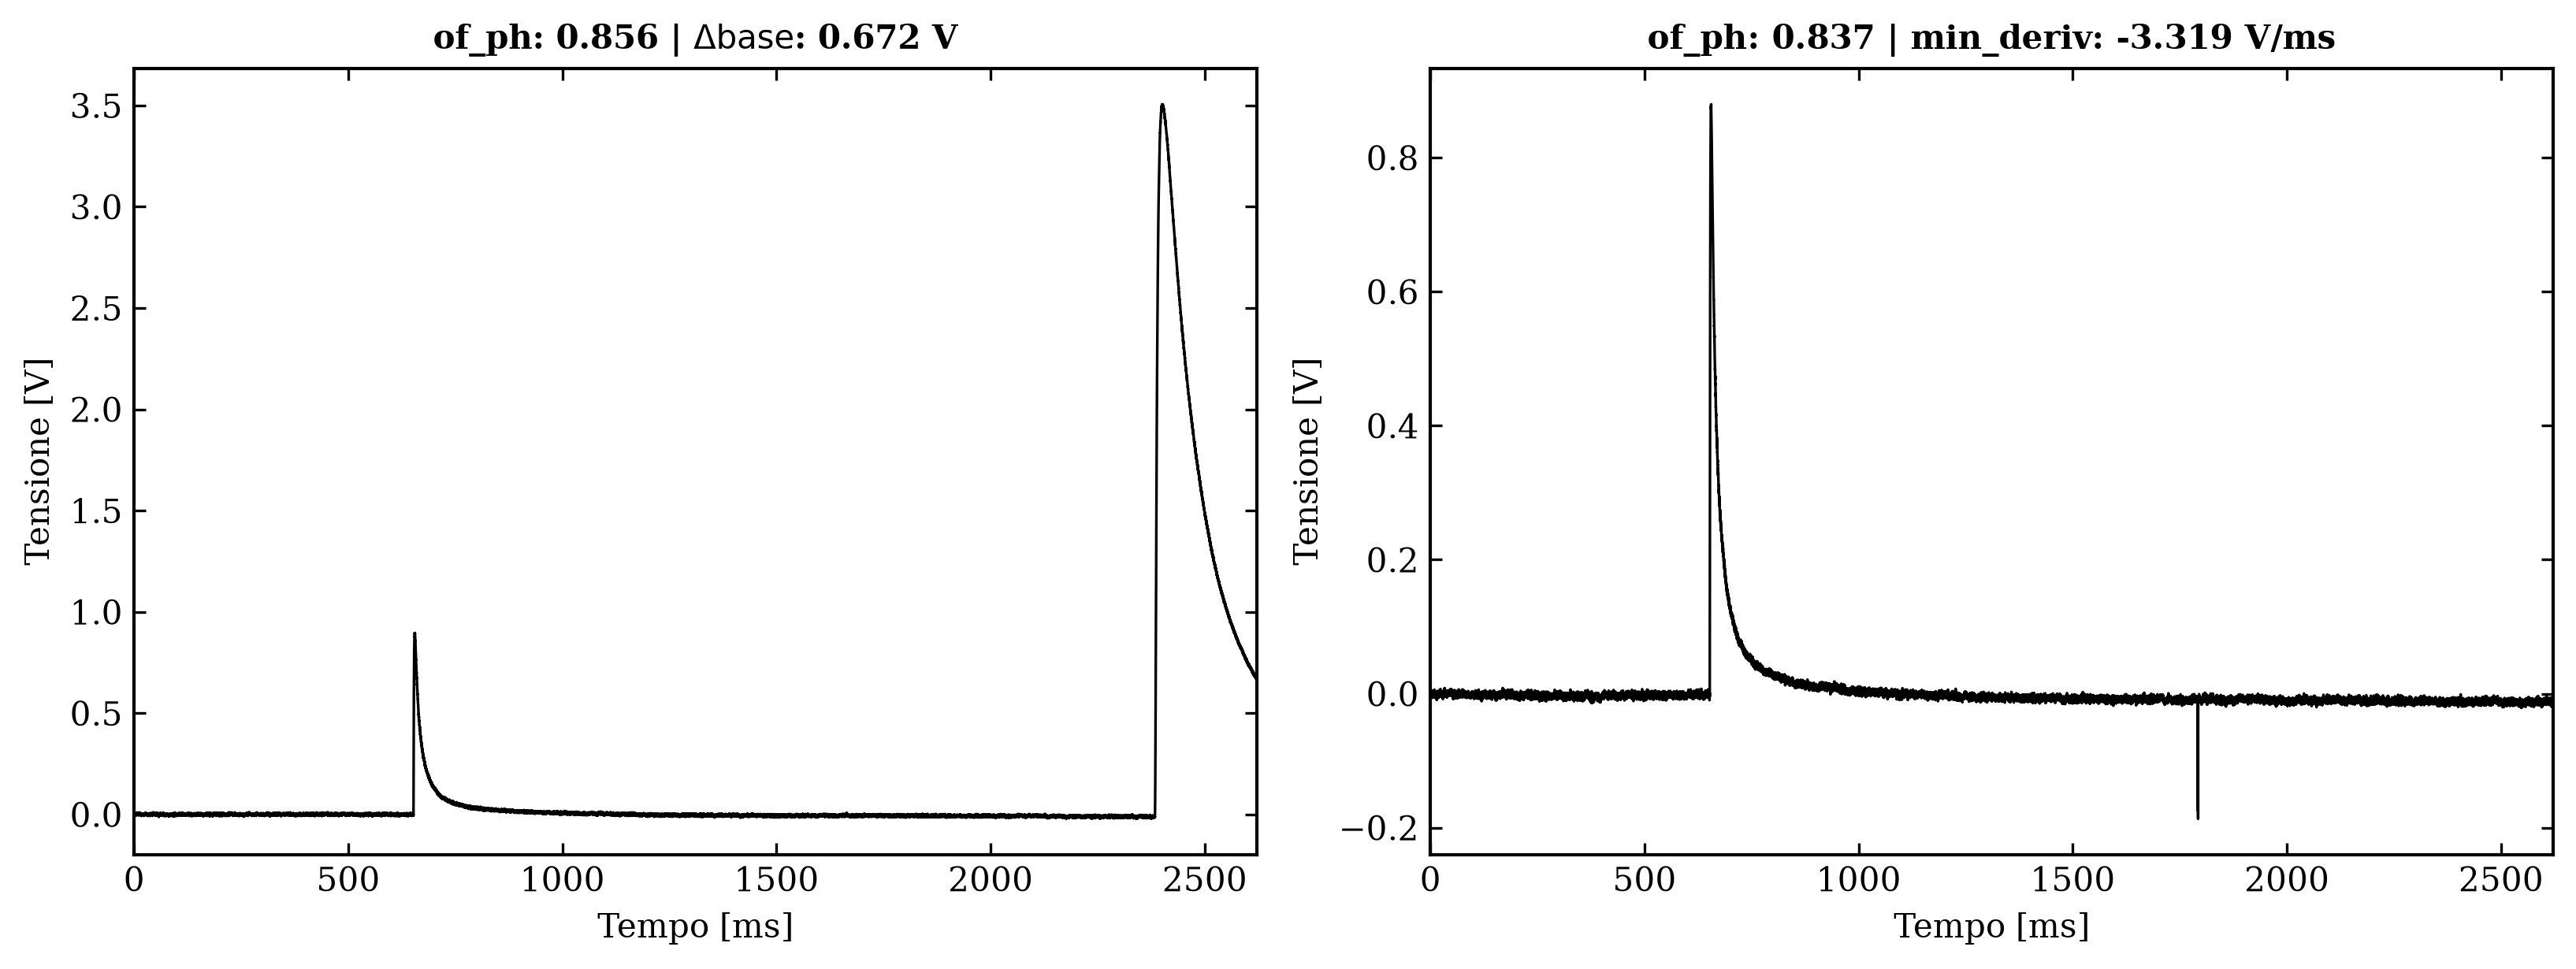
\includegraphics[width=0.9\textwidth]{figures/eventi_rigettati.png}
    \caption{Esempi di eventi fisici scartati dai tagli preliminari a causa di anomalie di baseline e problemi alla linearità del rivelatore: in particolare si nota il primo evento soggetto ad una elevata baseline difference dovuta ad un secondo evento verificatosi nella stessa finestra, mentre nel secondo caso una spike negativa dovuta probabilmente ad un'anomalai dell'elettronica.}
    \label{fig:eventi_rigettati}
\end{figure}

Tuttavia, questi tagli standard non sono in grado di intercettare i casi di \textit{pile-up}, in cui una seconda interazione avviene nella stessa finestra temporale senza alterare drasticamente la baseline finale. La presenza di un secondo picco altererebbe la forma media del template, compromettendo il calcolo dell'OF.

Per riconoscere ed eliminare questi eventi si impiega il \textbf{filtro di Savitzky-Golay}, un algoritmo che interpola localmente i punti con un polinomio di terzo grado, restituendo una traccia liscia. In particolare il polinomio è stato preso fittando 501 samples, 250 prima e 250 dopo il punto considerato. In seguito è stato preso il coefficiente costante del polinomio. Tale operazione è stata iterata per tutti i punti della finestra, ottenendo una forma d'onda in cui è stato abbattuto il rumore ad alta frequenza ma preservata la cuspide dell'impulso.
Sulla curva smussata viene applicato un algoritmo di ricerca dei massimi con due condizioni:
\begin{itemize}
    \item \textbf{Separazione temporale:} distanza minima tra picchi di $60\,\text{ms}$;
    \item \textbf{Prominenza minima:} ampiezza netta del picco di almeno $0.05\,\text{V}$.
\end{itemize}
Tale algoritmo non potrebbe essere applicato alla traccia grezza poiché intercetterebbe tutti i picchi dovuti alle fluttuazioni stocastiche del rumore.
Le tracce che manifestano più di un massimo valido vengono classificate come pile-up e scartate (Figura~\ref{fig:evento_rigettato_pileup}).

\begin{figure}[htbp]
    \centering
    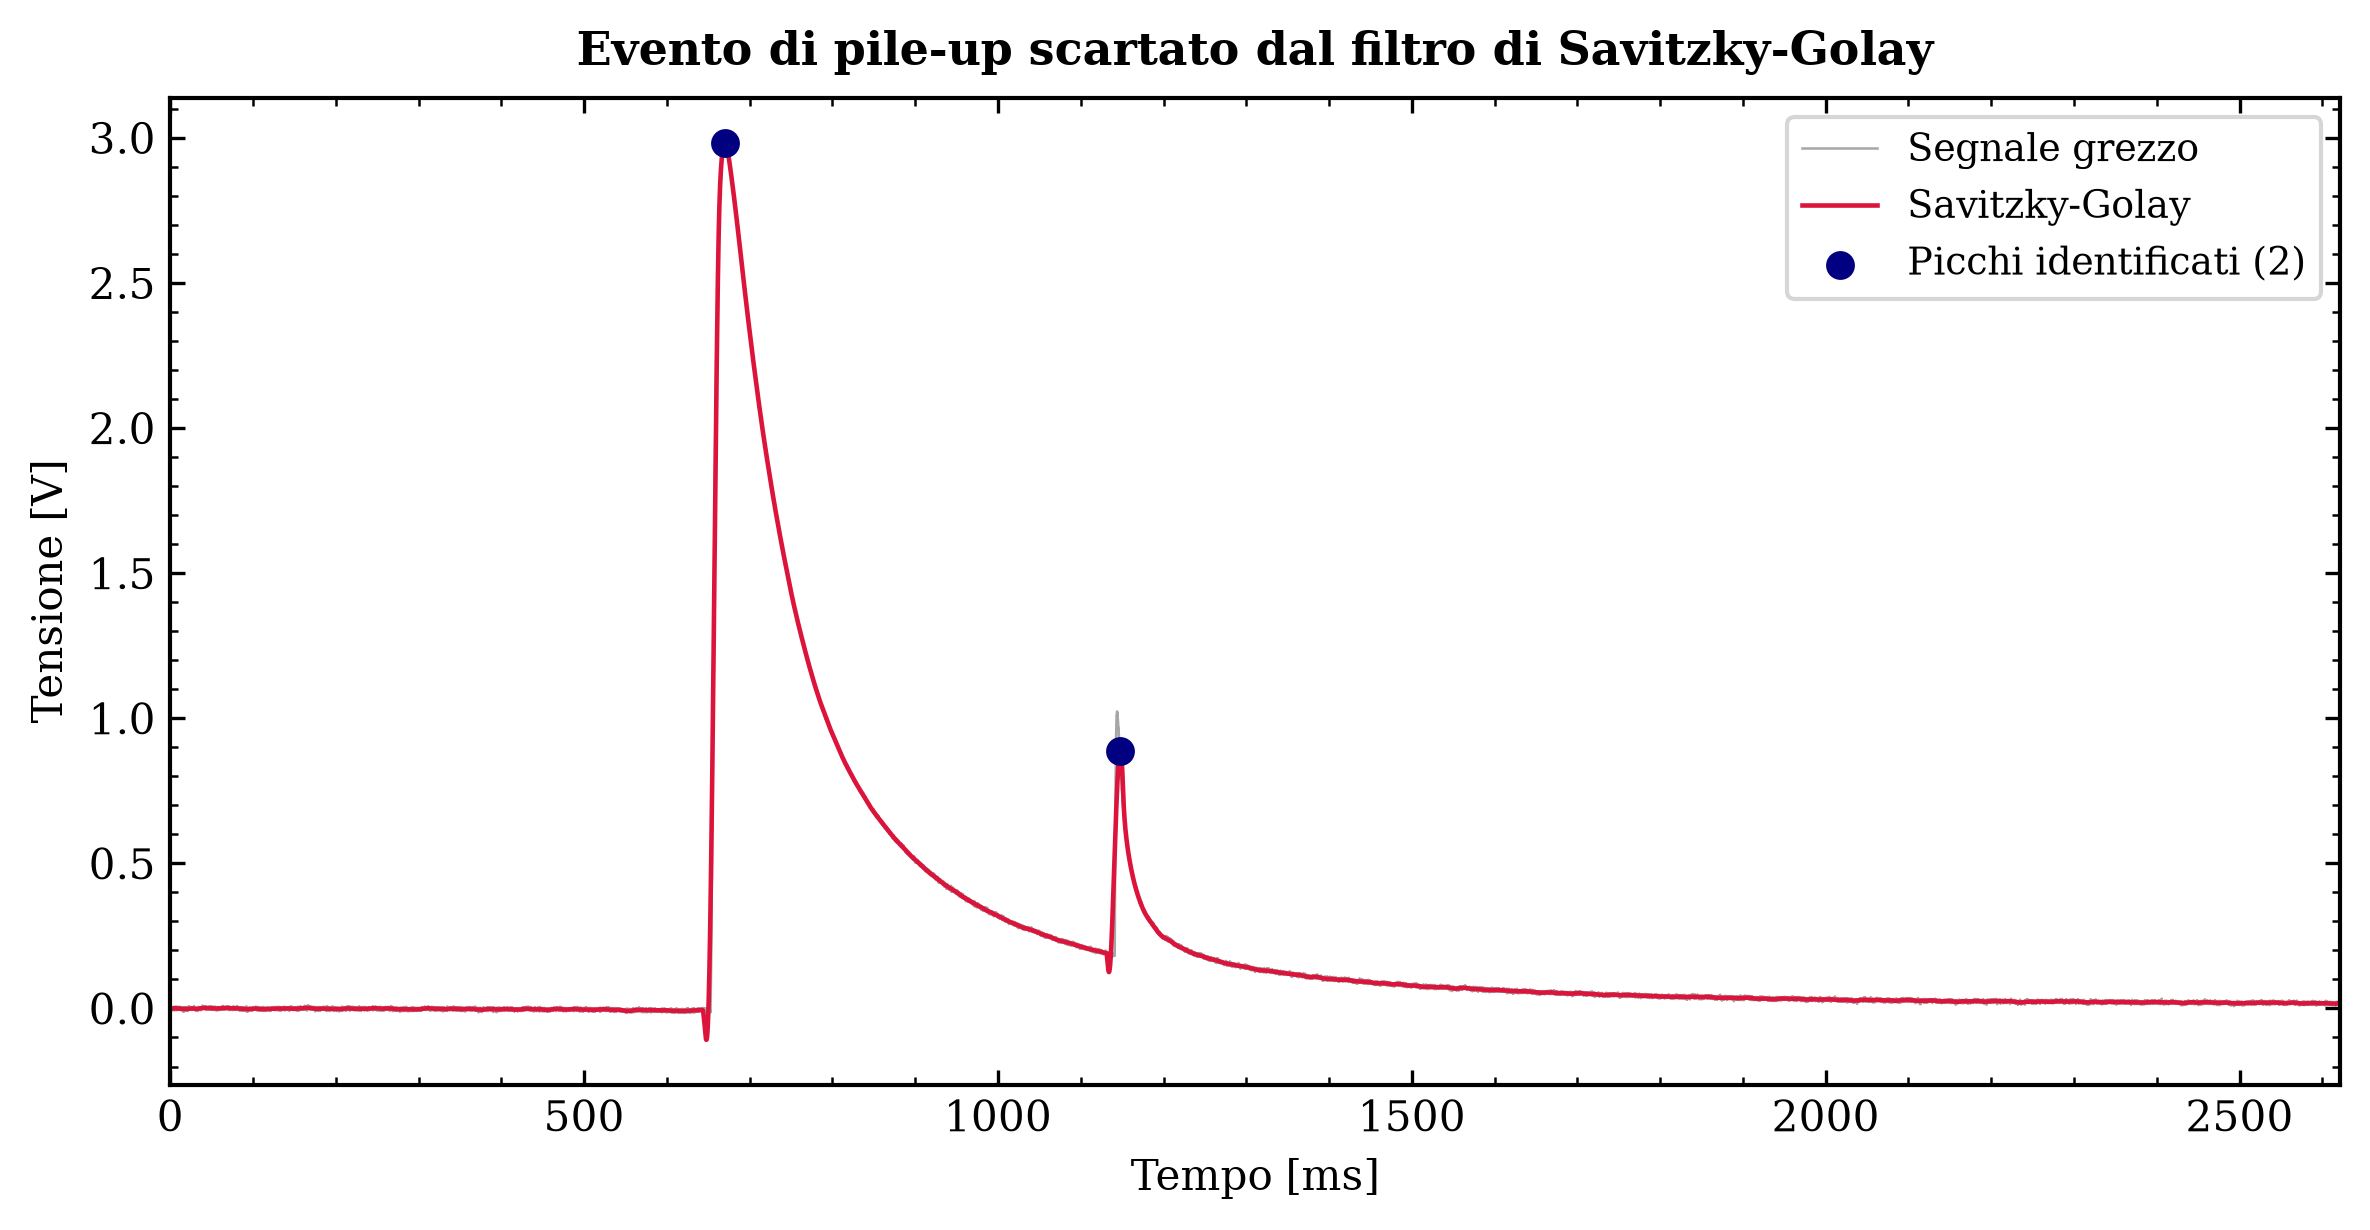
\includegraphics[width=0.88\textwidth]{figures/Esempio_Savitzky_Golay.png}
    \caption{Identificazione del pile-up tramite Savitzky-Golay: la curva smussata (in rosso) permette all'algoritmo di intercettare il secondo massimo locale ed escludere la traccia dal calcolo del template.}
    \label{fig:evento_rigettato_pileup}
\end{figure}

Mediando $337$ eventi di $^{55}\text{Fe}$ sopravvissuti ai tagli e normalizzando l'ampiezza al valore massimo unitario si ottiene il template fononico $s(t)$ (Figura~\ref{fig:confronto_templates}) e il corrispondente spettro di Fourier $S(f)$ (Figura~\ref{fig:FT_impulso_scremato}).

\begin{figure}[htbp]
        \centering
        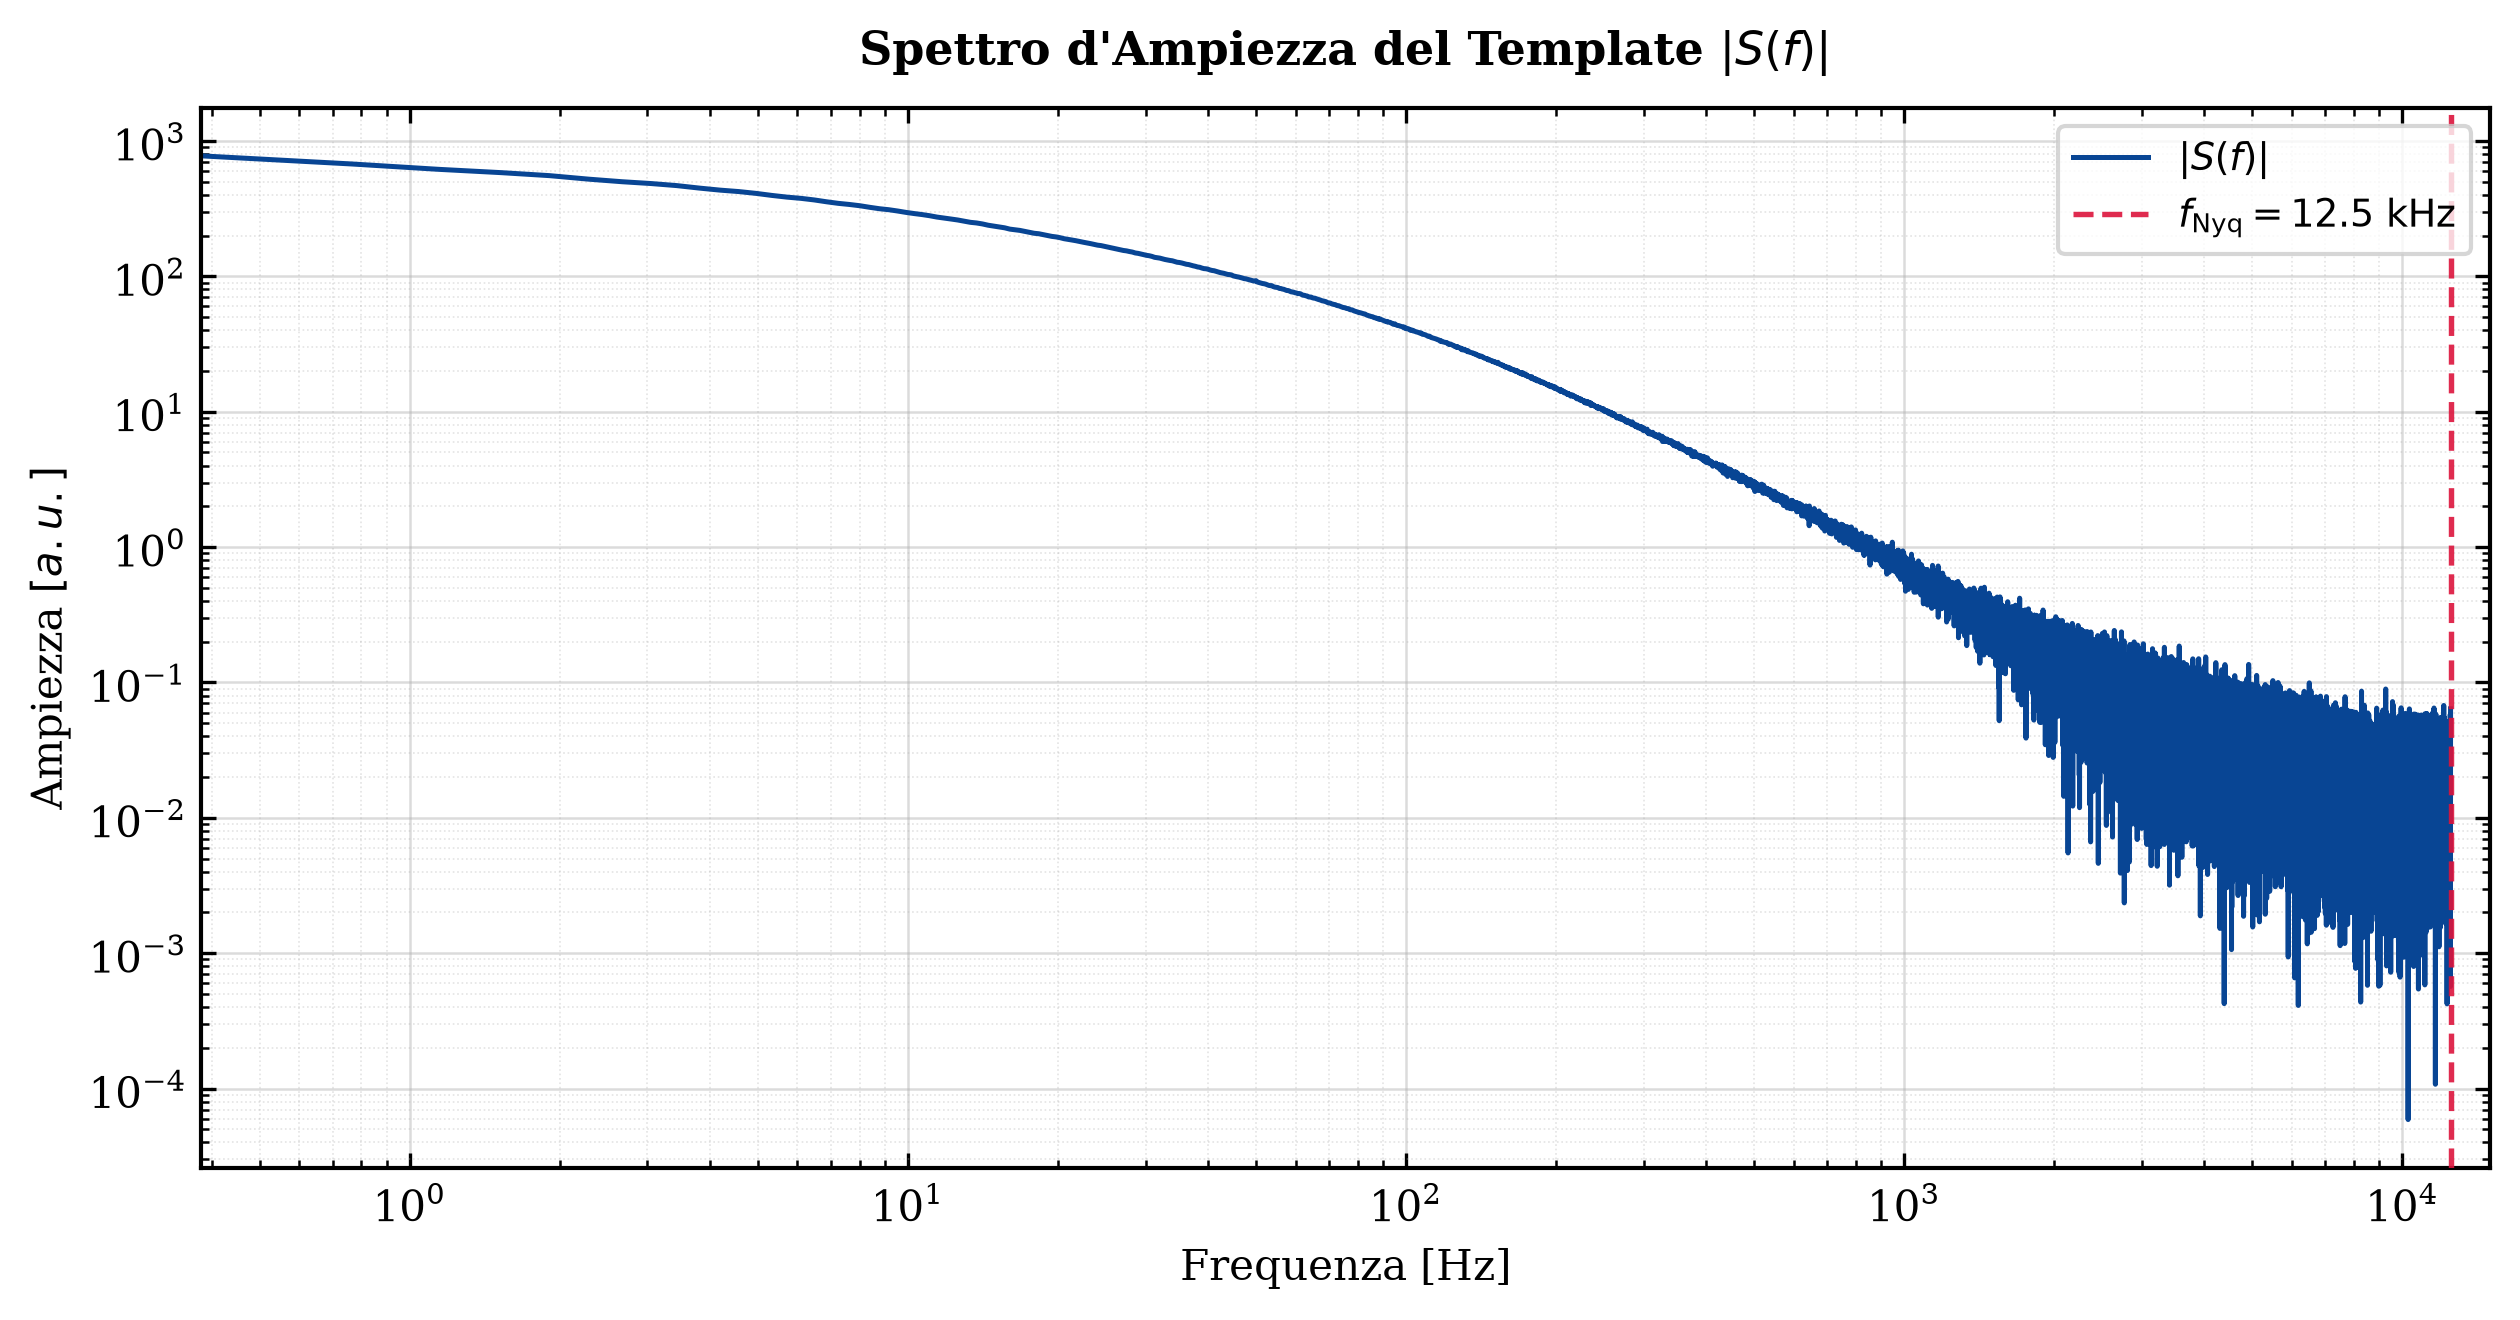
\includegraphics[width=0.85\linewidth]{figures/FT_impulso_scremato.png}
        \caption{Spettro di Fourier $S(f)$ del template fononico.}
        \label{fig:FT_impulso_scremato}
\end{figure}

% ------------------------------------------------------------------------------
\subsection{Template dei TestPulses e Confronto Morfologico}
\label{subsec:template_testpulse}

La risposta termica del rivelatore a un impulso di calore iniettato nell'heater non è del tutto identica a quella generata da una particella che colpisce il volume del cristallo. Sebbene entrambi i processi producano fononi termici, l'iniezione tramite heater avviene localmente sulla superficie e presenta una cinetica di diffusione leggermente differente.

Come illustrato nel confronto di Figura~\ref{fig:confronto_templates}, il TestPulse mostra un fronte di salita più dolce e un tempo di decadimento leggermente diverso rispetto all'impulso da particella. Per calibrare accuratamente i TestPulses senza introdurre disallineamenti di forma, è indispensabile costruire un template dedicato anche per essi.

\begin{figure}[htbp]
    \centering
    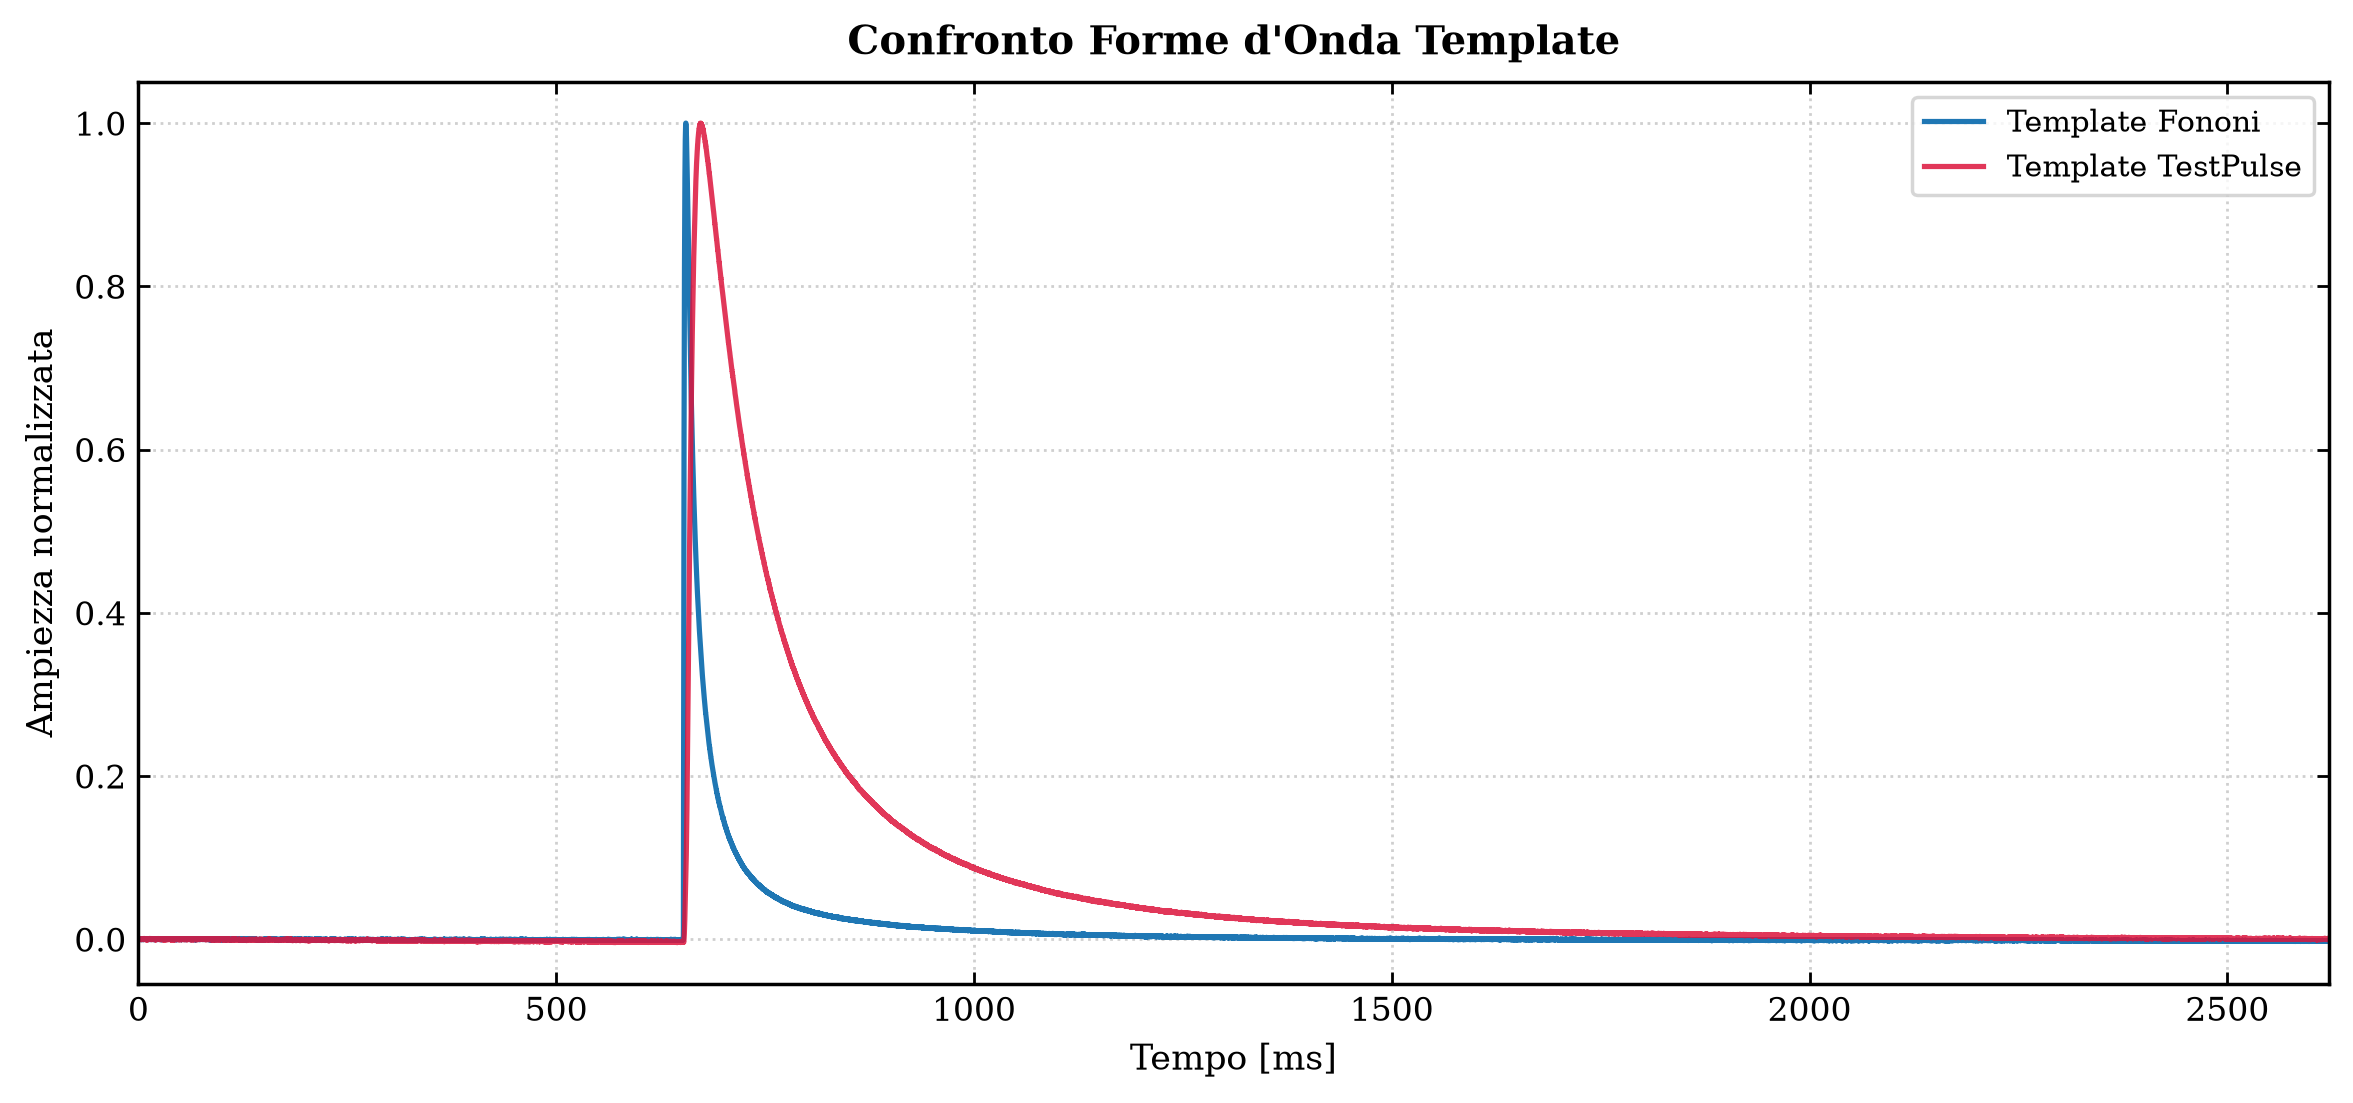
\includegraphics[width=0.85\textwidth]{figures/confronto_templates.png}
    \caption{Confronto normalizzato tra il template di particella ($^{55}\text{Fe}$) e il template ricavato dai TestPulses: l'impulso da particella presenta un tempo di salita più rapido.}
    \label{fig:confronto_templates}
\end{figure}

La procedura adottata per i TestPulses ricalca quella appena descritta: si selezionano impulsi non saturi generati a tensione costante ($V_{\text{inj}} = 1\,\text{V}$), si applicano i filtri su stabilità di baseline, assenza di pile-up e planarità della coda finale, e si media l'insieme delle tracce accettate normalizzando il picco a $1$.

% ==============================================================================
\section{Implementazione dell'Optimum Filter e Risultati}
\label{sec:applicazione_OF}
% ==============================================================================

Disponendo dell'NPS e del template di forma, la funzione di trasferimento $H(f)$ (Figura~\ref{fig:OF_complete}) viene utilizzata per estrarre l'esatta ampiezza di un evento secondo i seguenti passaggi:
\begin{enumerate}
    \item Si calcola la FT del segnale e la si moltiplica frequenza per frequenza per $H(f)$;
    \item Si esegue l'antitrasformata inversa (IFT) per tornare nel dominio del tempo;
    \item L'ampiezza dell'evento viene estratta dal picco del segnale filtrato, che risulta privo delle componenti oscillanti ad alta frequenza e delle interferenze a $50\,\text{Hz}$.
    \item L'evento viene ricostruito moltiplicando punto per punto il template per l'ampiezza ricostruita dal filtro.
\end{enumerate}

\begin{figure}[htbp]
    \centering
    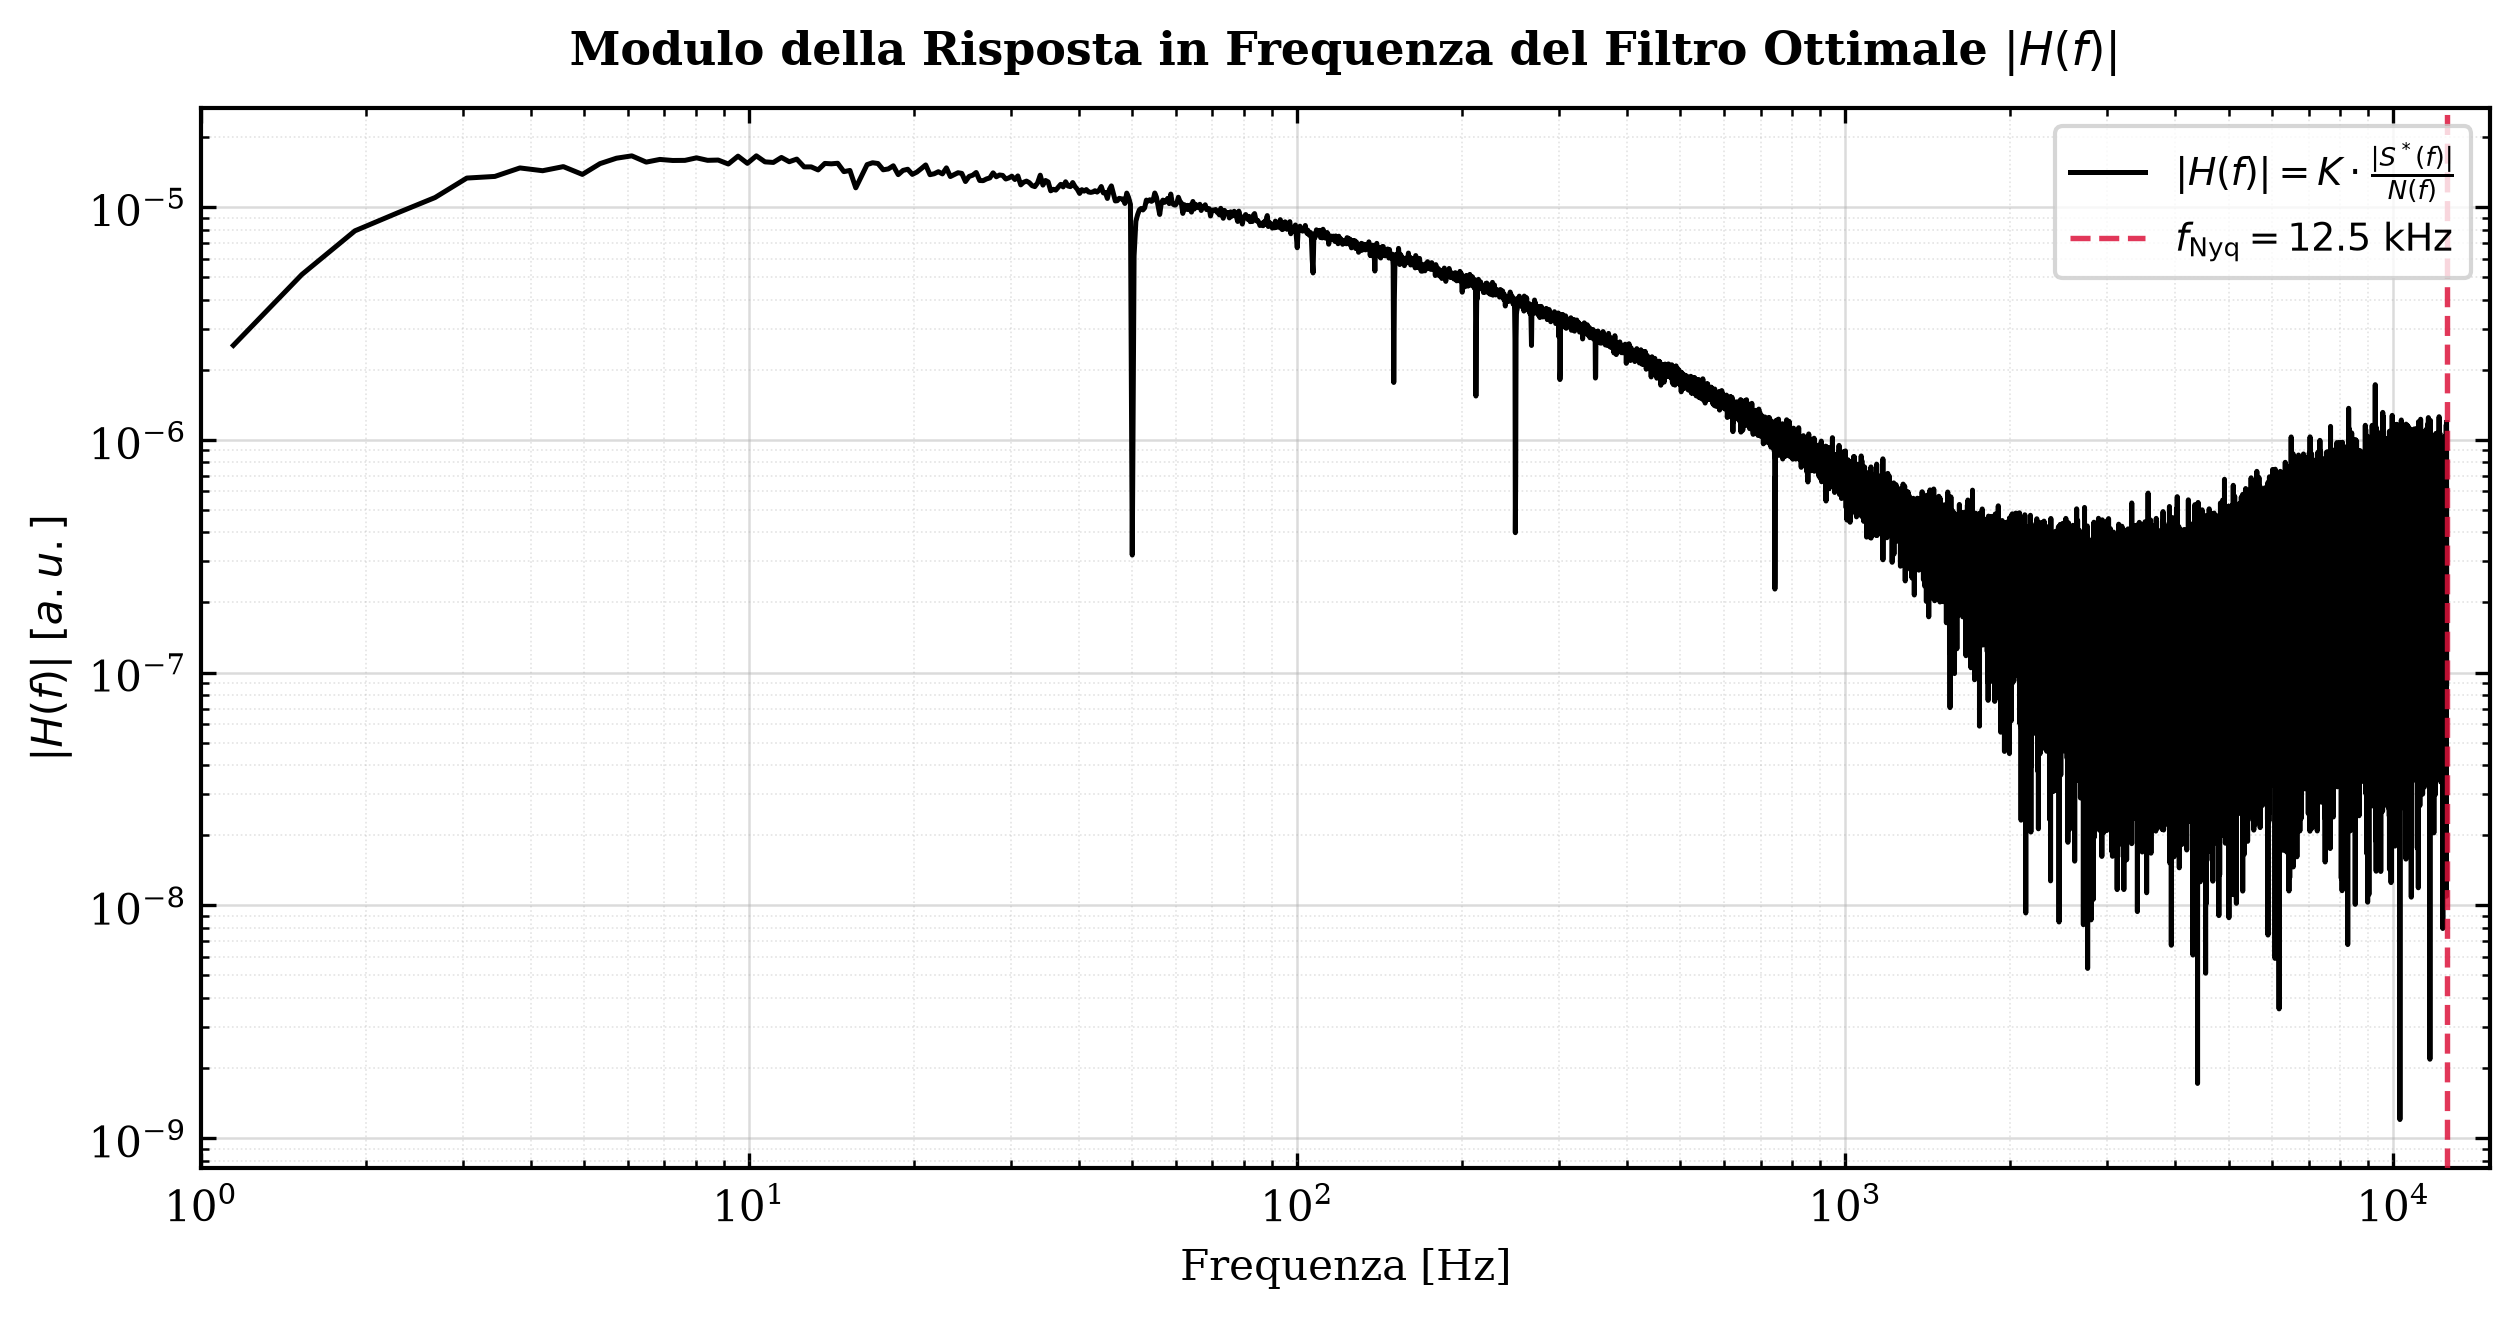
\includegraphics[width=0.8\textwidth]{figures/OF_rms.png}
    \caption{Modulo della funzione di trasferimento $H(f)$ dell'Optimum Filter per un evento di particella: si nota l'accentuata soppressione in corrispondenza del rumore di rete ($50\,\text{Hz}$) e alle alte frequenze.}
    \label{fig:OF_complete}
\end{figure}

Un esempio di applicazione su un impulso di piccola ampiezza ($V_{\text{inj}} = 0.5\,\text{V}$) è mostrato in Figura~\ref{fig:ricostruzione_TP}. La traccia grezza, inizialmente dominata dalle fluttuazioni casuali, viene pulita efficacemente dall'OF, consentendo una misura precisa e non distorta dell'altezza dell'impulso.

\begin{figure}[htbp]
    \centering
    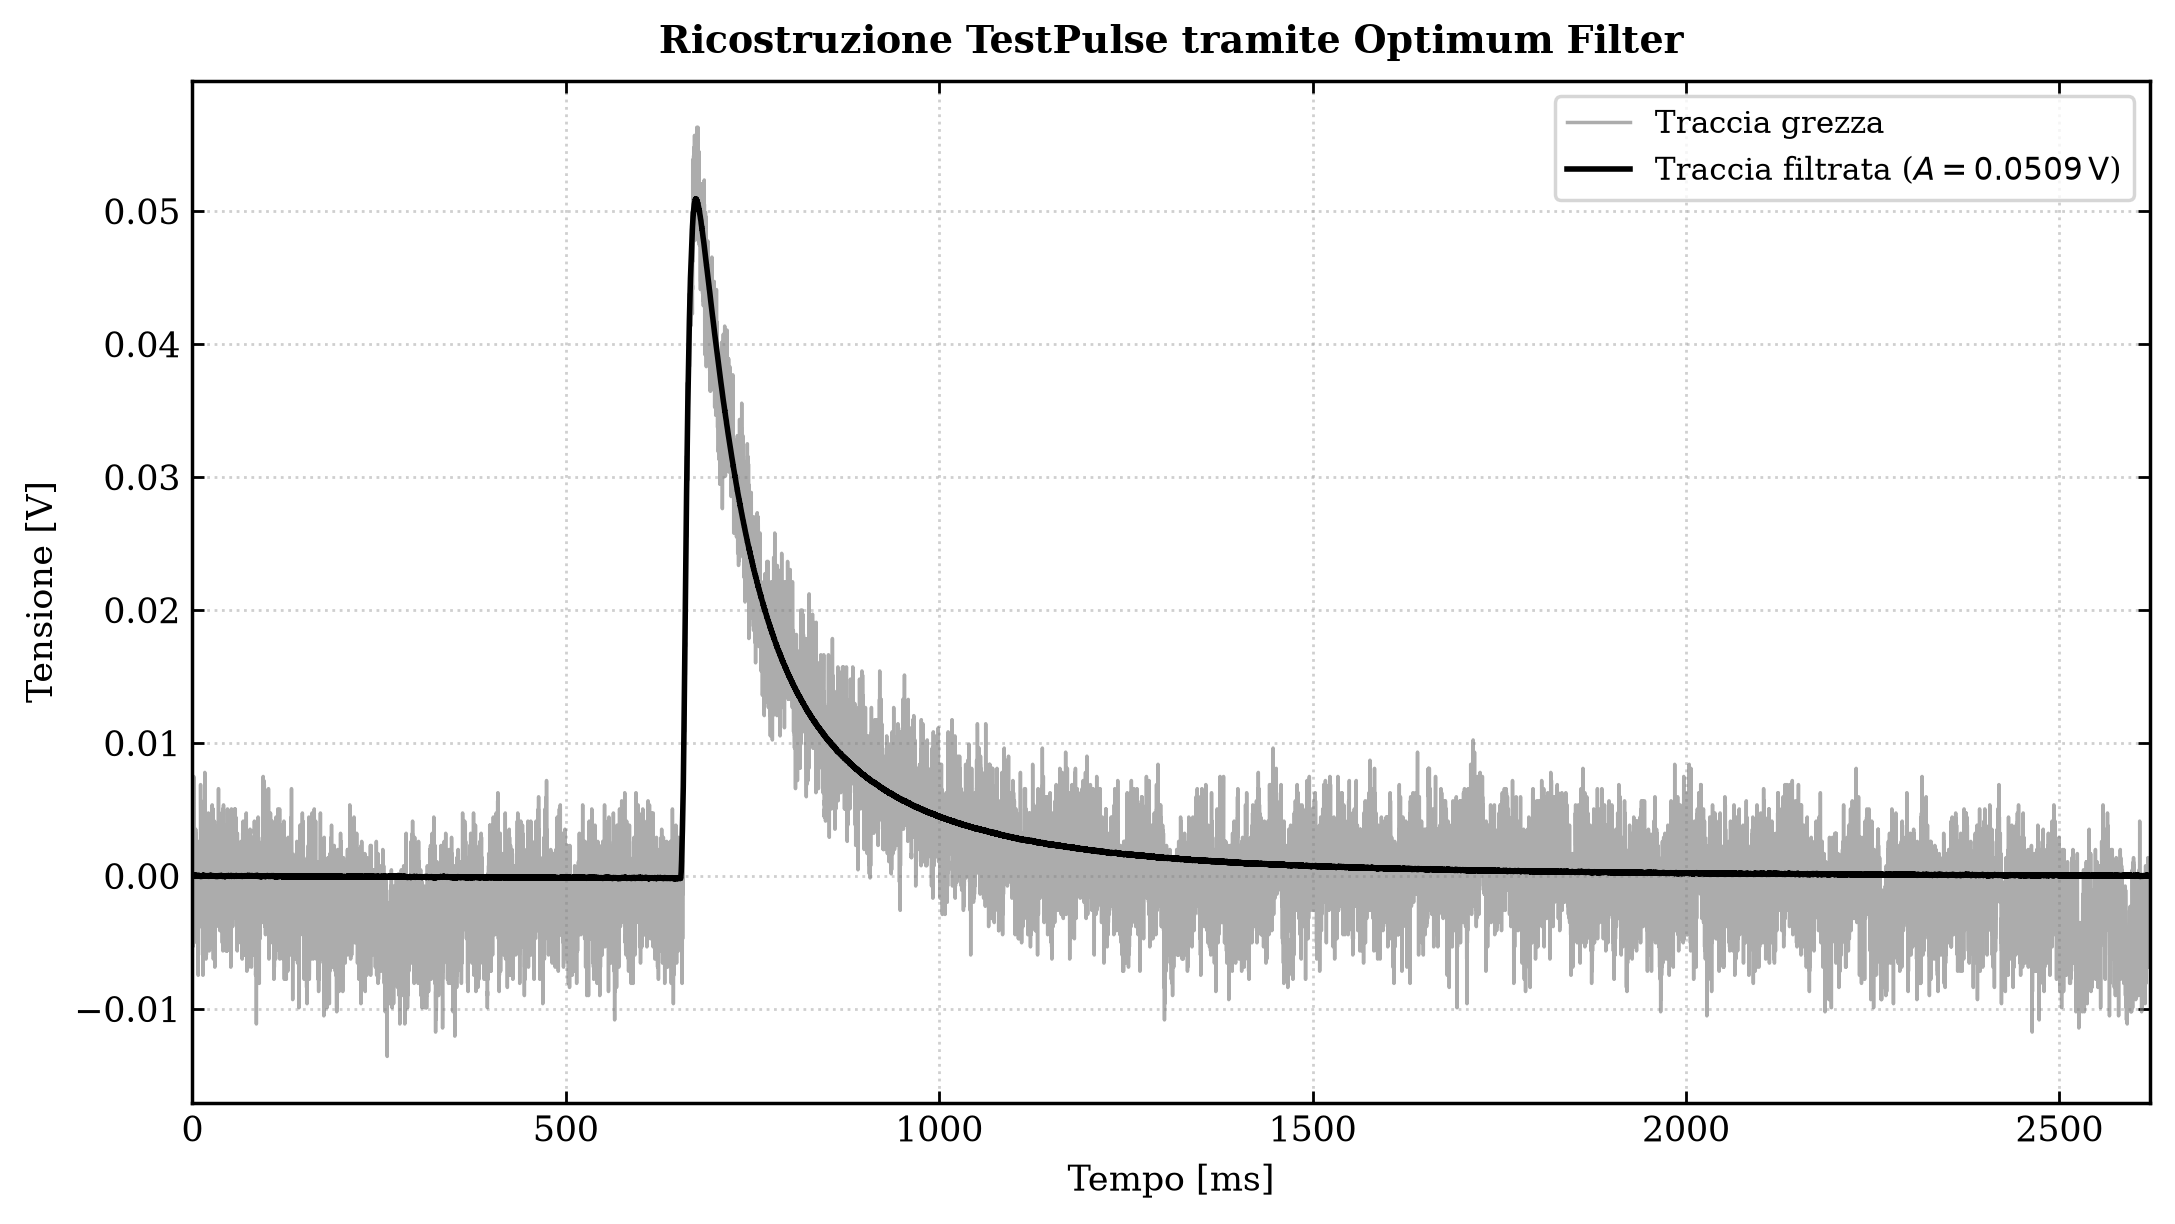
\includegraphics[width=0.7\textwidth]{figures/esempio_ric_TP.png}
    \caption{Applicazione dell'Optimum Filter a un TestPulse a bassa energia: confronto tra traccia grezza (grigio) e ricostruzione ottenuta scalando il template sull'ampiezza stimata (nero).}
    \label{fig:ricostruzione_TP}
\end{figure}

% ==============================================================================
\section{Rumore Residuo e Determinazione della Soglia di Trigger}
\label{sec:trigger_noise}
% ==============================================================================

to be continue...